\documentclass[ignorenonframetext,]{beamer}
\setbeamertemplate{caption}[numbered]
\setbeamertemplate{caption label separator}{: }
\setbeamercolor{caption name}{fg=normal text.fg}
\beamertemplatenavigationsymbolsempty
\usepackage{lmodern}
\usepackage{amssymb,amsmath}
\usepackage{ifxetex,ifluatex}
\usepackage{fixltx2e} % provides \textsubscript
\ifnum 0\ifxetex 1\fi\ifluatex 1\fi=0 % if pdftex
  \usepackage[T1]{fontenc}
  \usepackage[utf8]{inputenc}
\else % if luatex or xelatex
  \ifxetex
    \usepackage{mathspec}
  \else
    \usepackage{fontspec}
  \fi
  \defaultfontfeatures{Ligatures=TeX,Scale=MatchLowercase}
\fi
\usetheme[]{CambridgeUS}
\usecolortheme{beaver}
\usefonttheme{structurebold}
% use upquote if available, for straight quotes in verbatim environments
\IfFileExists{upquote.sty}{\usepackage{upquote}}{}
% use microtype if available
\IfFileExists{microtype.sty}{%
\usepackage{microtype}
\UseMicrotypeSet[protrusion]{basicmath} % disable protrusion for tt fonts
}{}
\newif\ifbibliography
\hypersetup{
            pdftitle={Das R-Paket tmap},
            pdfauthor={Jan-Philipp Kolb},
            pdfborder={0 0 0},
            breaklinks=true}
\urlstyle{same}  % don't use monospace font for urls
\usepackage{color}
\usepackage{fancyvrb}
\newcommand{\VerbBar}{|}
\newcommand{\VERB}{\Verb[commandchars=\\\{\}]}
\DefineVerbatimEnvironment{Highlighting}{Verbatim}{commandchars=\\\{\}}
% Add ',fontsize=\small' for more characters per line
\usepackage{framed}
\definecolor{shadecolor}{RGB}{248,248,248}
\newenvironment{Shaded}{\begin{snugshade}}{\end{snugshade}}
\newcommand{\KeywordTok}[1]{\textcolor[rgb]{0.13,0.29,0.53}{\textbf{#1}}}
\newcommand{\DataTypeTok}[1]{\textcolor[rgb]{0.13,0.29,0.53}{#1}}
\newcommand{\DecValTok}[1]{\textcolor[rgb]{0.00,0.00,0.81}{#1}}
\newcommand{\BaseNTok}[1]{\textcolor[rgb]{0.00,0.00,0.81}{#1}}
\newcommand{\FloatTok}[1]{\textcolor[rgb]{0.00,0.00,0.81}{#1}}
\newcommand{\ConstantTok}[1]{\textcolor[rgb]{0.00,0.00,0.00}{#1}}
\newcommand{\CharTok}[1]{\textcolor[rgb]{0.31,0.60,0.02}{#1}}
\newcommand{\SpecialCharTok}[1]{\textcolor[rgb]{0.00,0.00,0.00}{#1}}
\newcommand{\StringTok}[1]{\textcolor[rgb]{0.31,0.60,0.02}{#1}}
\newcommand{\VerbatimStringTok}[1]{\textcolor[rgb]{0.31,0.60,0.02}{#1}}
\newcommand{\SpecialStringTok}[1]{\textcolor[rgb]{0.31,0.60,0.02}{#1}}
\newcommand{\ImportTok}[1]{#1}
\newcommand{\CommentTok}[1]{\textcolor[rgb]{0.56,0.35,0.01}{\textit{#1}}}
\newcommand{\DocumentationTok}[1]{\textcolor[rgb]{0.56,0.35,0.01}{\textbf{\textit{#1}}}}
\newcommand{\AnnotationTok}[1]{\textcolor[rgb]{0.56,0.35,0.01}{\textbf{\textit{#1}}}}
\newcommand{\CommentVarTok}[1]{\textcolor[rgb]{0.56,0.35,0.01}{\textbf{\textit{#1}}}}
\newcommand{\OtherTok}[1]{\textcolor[rgb]{0.56,0.35,0.01}{#1}}
\newcommand{\FunctionTok}[1]{\textcolor[rgb]{0.00,0.00,0.00}{#1}}
\newcommand{\VariableTok}[1]{\textcolor[rgb]{0.00,0.00,0.00}{#1}}
\newcommand{\ControlFlowTok}[1]{\textcolor[rgb]{0.13,0.29,0.53}{\textbf{#1}}}
\newcommand{\OperatorTok}[1]{\textcolor[rgb]{0.81,0.36,0.00}{\textbf{#1}}}
\newcommand{\BuiltInTok}[1]{#1}
\newcommand{\ExtensionTok}[1]{#1}
\newcommand{\PreprocessorTok}[1]{\textcolor[rgb]{0.56,0.35,0.01}{\textit{#1}}}
\newcommand{\AttributeTok}[1]{\textcolor[rgb]{0.77,0.63,0.00}{#1}}
\newcommand{\RegionMarkerTok}[1]{#1}
\newcommand{\InformationTok}[1]{\textcolor[rgb]{0.56,0.35,0.01}{\textbf{\textit{#1}}}}
\newcommand{\WarningTok}[1]{\textcolor[rgb]{0.56,0.35,0.01}{\textbf{\textit{#1}}}}
\newcommand{\AlertTok}[1]{\textcolor[rgb]{0.94,0.16,0.16}{#1}}
\newcommand{\ErrorTok}[1]{\textcolor[rgb]{0.64,0.00,0.00}{\textbf{#1}}}
\newcommand{\NormalTok}[1]{#1}
\usepackage{longtable,booktabs}
\usepackage{caption}
% These lines are needed to make table captions work with longtable:
\makeatletter
\def\fnum@table{\tablename~\thetable}
\makeatother
\usepackage{graphicx,grffile}
\makeatletter
\def\maxwidth{\ifdim\Gin@nat@width>\linewidth\linewidth\else\Gin@nat@width\fi}
\def\maxheight{\ifdim\Gin@nat@height>\textheight0.8\textheight\else\Gin@nat@height\fi}
\makeatother
% Scale images if necessary, so that they will not overflow the page
% margins by default, and it is still possible to overwrite the defaults
% using explicit options in \includegraphics[width, height, ...]{}
\setkeys{Gin}{width=\maxwidth,height=\maxheight,keepaspectratio}

% Prevent slide breaks in the middle of a paragraph:
\widowpenalties 1 10000
\raggedbottom

\AtBeginPart{
  \let\insertpartnumber\relax
  \let\partname\relax
  \frame{\partpage}
}
\AtBeginSection{
  \ifbibliography
  \else
    \let\insertsectionnumber\relax
    \let\sectionname\relax
    \frame{\sectionpage}
  \fi
}
\AtBeginSubsection{
  \let\insertsubsectionnumber\relax
  \let\subsectionname\relax
  \frame{\subsectionpage}
}

\setlength{\parindent}{0pt}
\setlength{\parskip}{6pt plus 2pt minus 1pt}
\setlength{\emergencystretch}{3em}  % prevent overfull lines
\providecommand{\tightlist}{%
  \setlength{\itemsep}{0pt}\setlength{\parskip}{0pt}}
\setcounter{secnumdepth}{0}

\title{Das R-Paket tmap}
\author{Jan-Philipp Kolb}
\date{22 Oktober 2018}

\begin{document}
\frame{\titlepage}

\begin{frame}[fragile]{Das Paket
\href{https://cran.r-project.org/web/packages/tmap/index.html}{tmap}}

\begin{itemize}
\tightlist
\item
  Mit dem Paket
  \href{http://twitter.com/sharon000/status/593028906820599808/photo/1?ref_src=twsrc\%5Etfw}{\textbf{tmap}}
  kann man thematische Karten erzeugen
\item
  Die folgenden Beispiele sind auf der
  \href{https://cran.r-project.org/web/packages/tmap/vignettes/tmap-nutshell.html}{\textbf{Vignette}}
  des Paketes basiert.
\end{itemize}

\begin{Shaded}
\begin{Highlighting}[]
\KeywordTok{install.packages}\NormalTok{(}\StringTok{"tmap"}\NormalTok{)}
\end{Highlighting}
\end{Shaded}

\begin{Shaded}
\begin{Highlighting}[]
\KeywordTok{library}\NormalTok{(tmap)}
\end{Highlighting}
\end{Shaded}

\end{frame}

\begin{frame}[fragile]{Schnelle thematische Karte}

\begin{itemize}
\item
  Mit dem Befehl
  \href{https://cran.r-project.org/web/packages/tmap/vignettes/tmap-nutshell.html}{\textbf{qtm}}
  kann man eine schnelle thematische Karte erzeugen
\item
  Beispiel aus der
  \href{https://cran.r-project.org/web/packages/tmap/vignettes/tmap-nutshell.html}{\textbf{Vignette}}
  zum Paket \texttt{tmap}
\end{itemize}

\begin{Shaded}
\begin{Highlighting}[]
\KeywordTok{data}\NormalTok{(Europe)}
\KeywordTok{qtm}\NormalTok{(Europe)}
\end{Highlighting}
\end{Shaded}

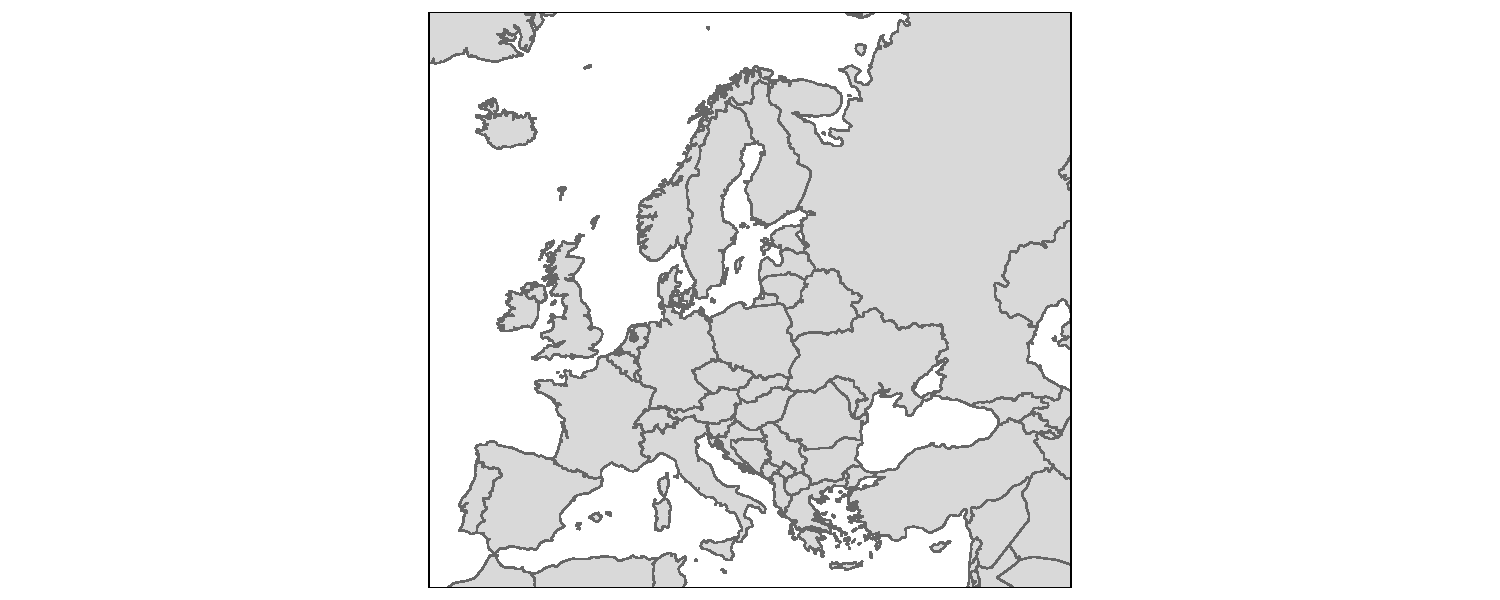
\includegraphics{tmap_files/figure-beamer/unnamed-chunk-4-1.pdf}

\end{frame}

\begin{frame}{Der Europa-Datensatz}

\begin{longtable}[]{@{}lllll@{}}
\toprule
& iso\_a3 & name & sovereignt & continent\tabularnewline
\midrule
\endhead
5 & ALB & Albania & Albania & Europe\tabularnewline
6 & ALA & Aland & Finland & Europe\tabularnewline
7 & AND & Andorra & Andorra & Europe\tabularnewline
10 & ARM & Armenia & Armenia & Asia\tabularnewline
17 & AUT & Austria & Austria & Europe\tabularnewline
18 & AZE & Azerbaijan & Azerbaijan & Asia\tabularnewline
20 & BEL & Belgium & Belgium & Europe\tabularnewline
24 & BGR & Bulgaria & Bulgaria & Europe\tabularnewline
27 & BIH & Bosnia and Herz. & Bosnia and Herzegovina &
Europe\tabularnewline
29 & BLR & Belarus & Belarus & Europe\tabularnewline
\bottomrule
\end{longtable}

\end{frame}

\begin{frame}[fragile]{Um mehr Farbe in die Karte zu bekommen}

\begin{itemize}
\tightlist
\item
  Visualisierung von
  \href{http://www.naturalearthdata.com/}{\textbf{Natural Earth}} Daten
\end{itemize}

\begin{Shaded}
\begin{Highlighting}[]
\KeywordTok{qtm}\NormalTok{(Europe, }\DataTypeTok{fill=}\StringTok{"gdp_cap_est"}\NormalTok{)}
\end{Highlighting}
\end{Shaded}

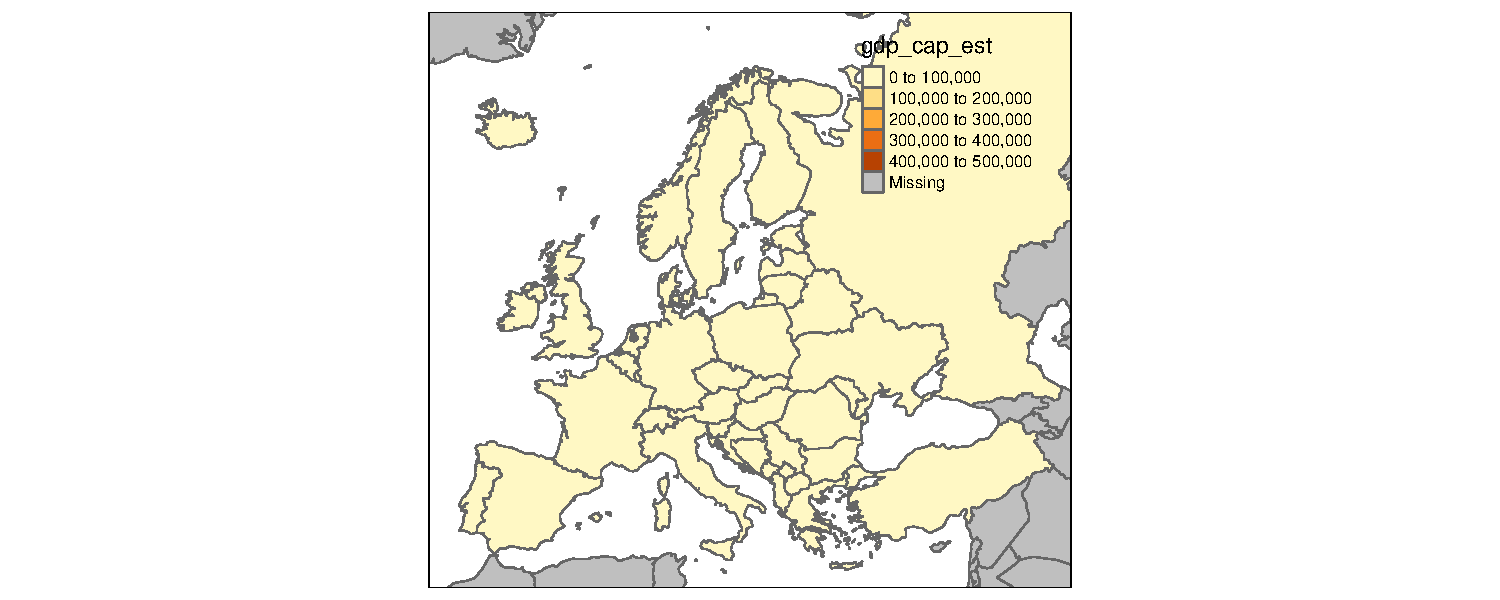
\includegraphics{tmap_files/figure-beamer/unnamed-chunk-8-1.pdf}

\end{frame}

\begin{frame}[fragile]{Eine Karte mit Text}

\begin{Shaded}
\begin{Highlighting}[]
\KeywordTok{qtm}\NormalTok{(Europe, }\DataTypeTok{fill=}\StringTok{"gdp_cap_est"}\NormalTok{, }\DataTypeTok{text=}\StringTok{"iso_a3"}\NormalTok{)}
\end{Highlighting}
\end{Shaded}

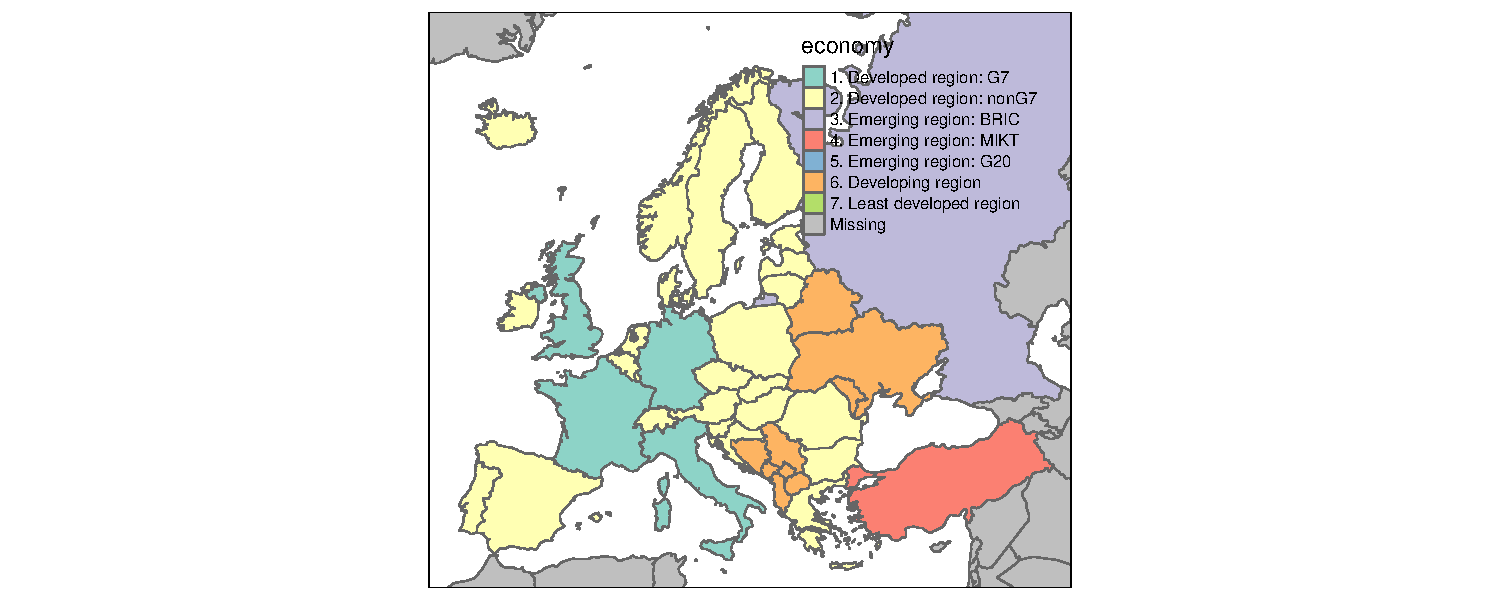
\includegraphics{tmap_files/figure-beamer/unnamed-chunk-9-1.pdf}

\end{frame}

\begin{frame}[fragile]{Dieses Schema passt besser:}

\begin{block}{\href{https://en.wikipedia.org/wiki/Population_density}{\textbf{Bevölkerungsdichte}}}

\begin{Shaded}
\begin{Highlighting}[]
\KeywordTok{qtm}\NormalTok{(Europe, }\DataTypeTok{fill=}\StringTok{"gdp_cap_est"}\NormalTok{, }\DataTypeTok{text=}\StringTok{"iso_a3"}\NormalTok{, }
    \DataTypeTok{text.size=}\StringTok{"AREA"}\NormalTok{, }\DataTypeTok{root=}\DecValTok{5}\NormalTok{, }\DataTypeTok{fill.title=}\StringTok{"GDP per capita"}\NormalTok{, }
    \DataTypeTok{fill.textNA=}\StringTok{"Non-European countries"}\NormalTok{, }\DataTypeTok{theme=}\StringTok{"Europe"}\NormalTok{)}
\end{Highlighting}
\end{Shaded}

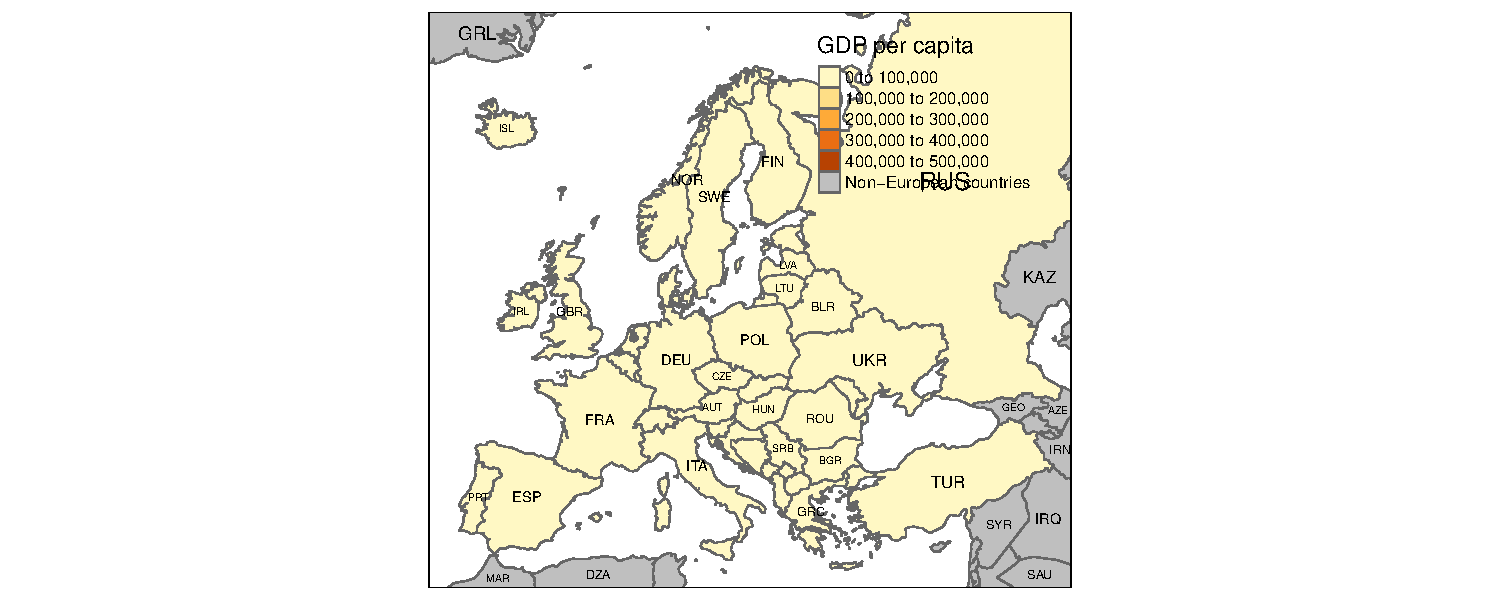
\includegraphics{tmap_files/figure-beamer/unnamed-chunk-10-1.pdf}

\end{block}

\end{frame}

\begin{frame}{Themen des Europa-Datensatzes}

\begin{itemize}
\tightlist
\item
  \href{http://userpage.chemie.fu-berlin.de/diverse/doc/ISO_3166.html}{\textbf{ISO
  Klassifikation}}
\item
  Ländername
\item
  Ist das Land Teil Europas?
\item
  Fläche, Bevölkerung, Bevölkerungsdichte,
\item
  \href{https://en.wikipedia.org/wiki/Gross_domestic_product}{\textbf{Bruttoinlandsprodukt}}
\item
  Bruttoinlandsprodukt
  \href{https://en.wikipedia.org/wiki/List_of_countries_by_GDP_\%28PPP\%29_per_capita}{\textbf{zu
  Kaufkraftparitäten}}
\item
  Ökonomie, Einkommensgruppe
\end{itemize}

\end{frame}

\begin{frame}{Der Europa Datensatz - Variablen und was dahinter steckt}

\begin{longtable}[]{@{}llllll@{}}
\toprule
& iso\_a3 & name & sovereignt & continent & part\tabularnewline
\midrule
\endhead
5 & ALB & Albania & Albania & Europe & Southern Europe\tabularnewline
6 & ALA & Aland & Finland & Europe & Northern Europe\tabularnewline
7 & AND & Andorra & Andorra & Europe & Southern Europe\tabularnewline
10 & ARM & Armenia & Armenia & Asia & NA\tabularnewline
17 & AUT & Austria & Austria & Europe & Western Europe\tabularnewline
18 & AZE & Azerbaijan & Azerbaijan & Asia & NA\tabularnewline
20 & BEL & Belgium & Belgium & Europe & Western Europe\tabularnewline
24 & BGR & Bulgaria & Bulgaria & Europe & Eastern Europe\tabularnewline
\bottomrule
\end{longtable}

\end{frame}

\begin{frame}[fragile]{Die Variable \texttt{continent}}

\begin{Shaded}
\begin{Highlighting}[]
\KeywordTok{qtm}\NormalTok{(Europe, }\DataTypeTok{fill=}\StringTok{"continent"}\NormalTok{)}
\end{Highlighting}
\end{Shaded}

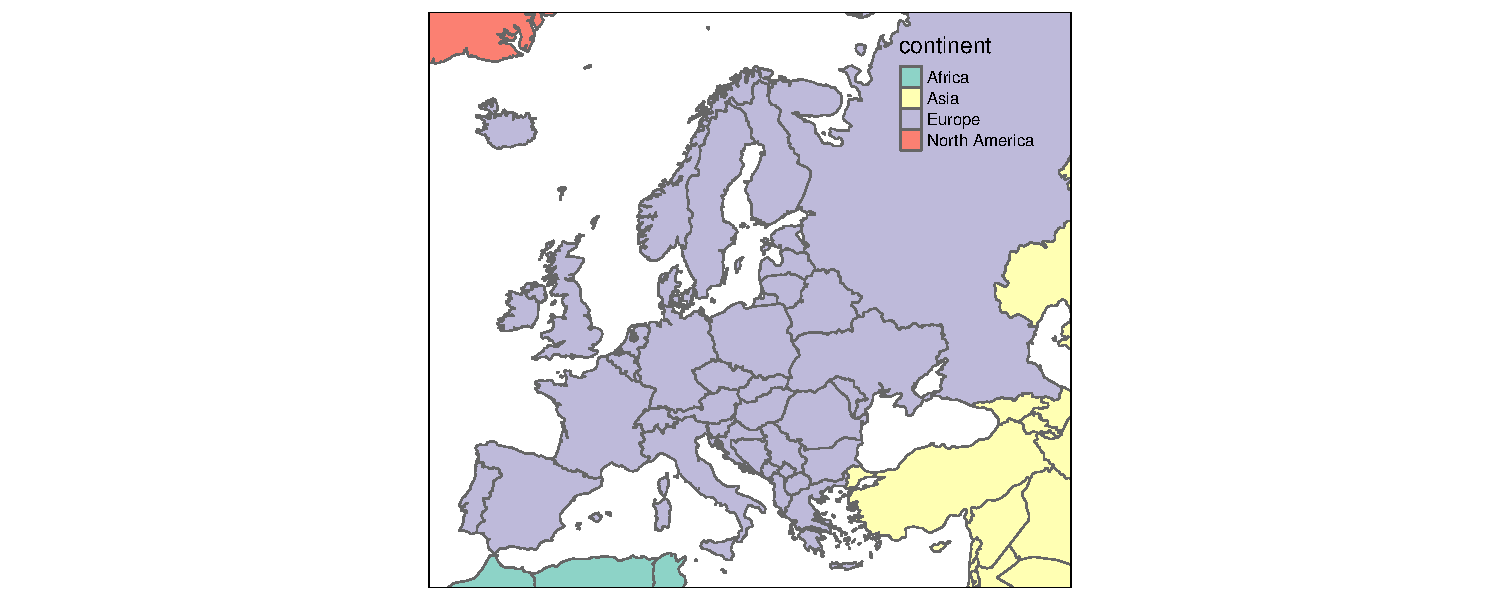
\includegraphics{tmap_files/figure-beamer/unnamed-chunk-14-1.pdf}

\end{frame}

\begin{frame}[fragile]{Die Variable \texttt{part}}

\begin{Shaded}
\begin{Highlighting}[]
\KeywordTok{qtm}\NormalTok{(Europe, }\DataTypeTok{fill=}\StringTok{"part"}\NormalTok{,}\DataTypeTok{fill.title=}\StringTok{"Teil von Europa"}\NormalTok{)}
\end{Highlighting}
\end{Shaded}


\includegraphics{tmap_files/figure-beamer/unnamed-chunk-15-1.pdf}

\end{frame}

\begin{frame}[fragile]{Die Variable \texttt{area}}

\begin{Shaded}
\begin{Highlighting}[]
\KeywordTok{qtm}\NormalTok{(Europe, }\DataTypeTok{fill=}\StringTok{"area"}\NormalTok{) }\CommentTok{# Russia is huge}
\end{Highlighting}
\end{Shaded}

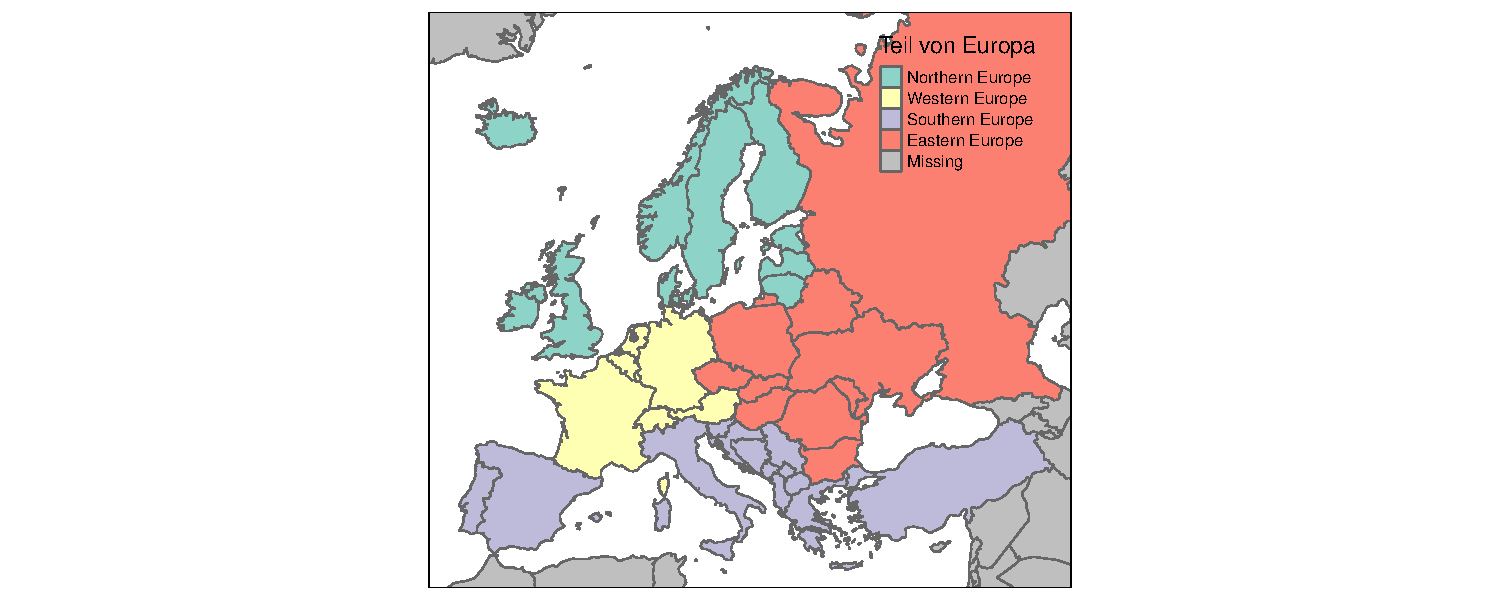
\includegraphics{tmap_files/figure-beamer/unnamed-chunk-16-1.pdf}

\end{frame}

\begin{frame}[fragile]{Bevölkerung}

\begin{Shaded}
\begin{Highlighting}[]
\KeywordTok{qtm}\NormalTok{(Europe, }\DataTypeTok{fill=}\StringTok{"pop_est"}\NormalTok{,}\DataTypeTok{fill.title=}\StringTok{"Population"}\NormalTok{) }
\end{Highlighting}
\end{Shaded}

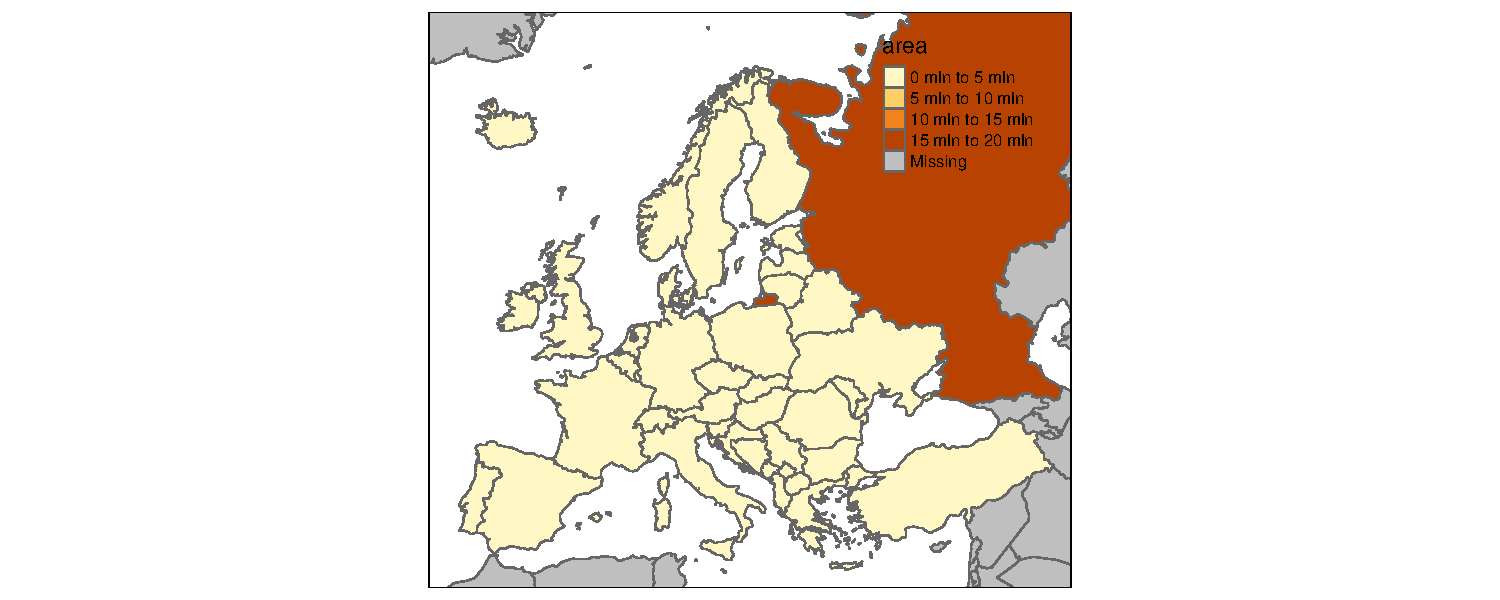
\includegraphics{tmap_files/figure-beamer/unnamed-chunk-17-1.pdf}

\end{frame}

\begin{frame}[fragile]{Ökonomie}

\begin{Shaded}
\begin{Highlighting}[]
\KeywordTok{qtm}\NormalTok{(Europe, }\DataTypeTok{fill=}\StringTok{"economy"}\NormalTok{) }
\end{Highlighting}
\end{Shaded}

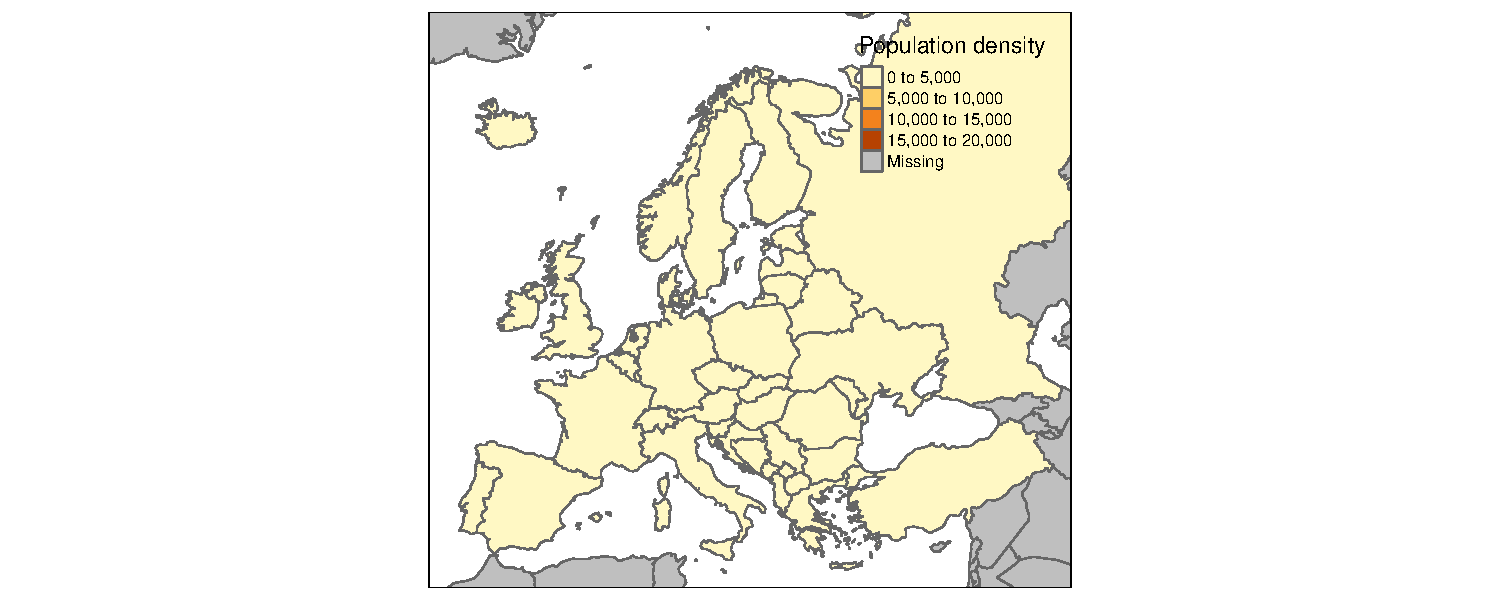
\includegraphics{tmap_files/figure-beamer/unnamed-chunk-19-1.pdf}

\end{frame}

\begin{frame}[fragile]{Einkommensgruppe}

\begin{Shaded}
\begin{Highlighting}[]
\KeywordTok{qtm}\NormalTok{(Europe, }\DataTypeTok{fill=}\StringTok{"income_grp"}\NormalTok{,}\DataTypeTok{fill.title=}\StringTok{"Income group"}\NormalTok{) }
\end{Highlighting}
\end{Shaded}


\includegraphics{tmap_files/figure-beamer/unnamed-chunk-20-1.pdf}

\end{frame}

\begin{frame}{Der Welt-Datensatz im Paket \texttt{tmap}}

\begin{longtable}[]{@{}llllllrrrrrllrrr@{}}
\toprule
& iso\_a3 & name & sovereignt & continent & subregion & area & pop\_est
& pop\_est\_dens & gdp\_md\_est & gdp\_cap\_est & economy & income\_grp
& life\_exp & well\_being & HPI\tabularnewline
\midrule
\endhead
2 & AFG & Afghanistan & Afghanistan & Asia & Southern Asia & 652860.000
& 28400000 & 43.5009037 & 22270 & 784.1549 & 7. Least developed region &
5. Low income & 48.7 & 4.758381 & 36.75366\tabularnewline
3 & AGO & Angola & Angola & Africa & Middle Africa & 1246700.000 &
12799293 & 10.2665381 & 110300 & 8617.6635 & 7. Least developed region &
3. Upper middle income & 51.1 & 4.206092 & 33.20143\tabularnewline
5 & ALB & Albania & Albania & Europe & Southern Europe & 27400.000 &
3639453 & 132.8267518 & 21810 & 5992.6588 & 6. Developing region & 4.
Lower middle income & 76.9 & 5.268937 & 54.05118\tabularnewline
8 & ARE & United Arab Emirates & United Arab Emirates & Asia & Western
Asia & 83600.000 & 4798491 & 57.3982177 & 184300 & 38407.9078 & 6.
Developing region & 2. High income: nonOECD & 76.5 & 7.196803 &
31.77827\tabularnewline
9 & ARG & Argentina & Argentina & South America & South America &
2736690.000 & 40913584 & 14.9500250 & 573900 & 14027.1261 & 5. Emerging
region: G20 & 3. Upper middle income & 75.9 & 6.441067 &
54.05504\tabularnewline
10 & ARM & Armenia & Armenia & Asia & Western Asia & 28470.000 & 2967004
& 104.2151036 & 18770 & 6326.2469 & 6. Developing region & 4. Lower
middle income & 74.2 & 4.367811 & 46.00319\tabularnewline
12 & ATA & Antarctica & Antarctica & Antarctica & Antarctica &
10866664.407 & 3802 & 0.0003499 & NA & NA & 6. Developing region & 2.
High income: nonOECD & NA & NA & NA\tabularnewline
14 & ATF & Fr. S. Antarctic Lands & France & Seven seas (open ocean) &
Seven seas (open ocean) & 6187.205 & 140 & 0.0226273 & 16 & 114285.7143
& 6. Developing region & 2. High income: nonOECD & NA & NA &
NA\tabularnewline
16 & AUS & Australia & Australia & Oceania & Australia and New Zealand &
7682300.000 & 21262641 & 2.7677442 & 800200 & 37634.0832 & 2. Developed
region: nonG7 & 1. High income: OECD & 81.9 & 7.405616 &
41.97981\tabularnewline
17 & AUT & Austria & Austria & Europe & Western Europe & 82409.000 &
8210281 & 99.6284508 & 329500 & 40132.6093 & 2. Developed region: nonG7
& 1. High income: OECD & 80.9 & 7.346036 & 47.08514\tabularnewline
18 & AZE & Azerbaijan & Azerbaijan & Asia & Western Asia & 82658.000 &
8238672 & 99.6718043 & 77610 & 9420.2075 & 6. Developing region & 3.
Upper middle income & 70.7 & 4.218611 & 40.88457\tabularnewline
19 & BDI & Burundi & Burundi & Africa & Eastern Africa & 25680.000 &
8988091 & 350.0035436 & 3102 & 345.1233 & 7. Least developed region & 5.
Low income & 50.4 & 3.791681 & 30.51501\tabularnewline
20 & BEL & Belgium & Belgium & Europe & Western Europe & 30280.000 &
10414336 & 343.9344782 & 389300 & 37381.1638 & 2. Developed region:
nonG7 & 1. High income: OECD & 80.0 & 6.853514 & 37.09053\tabularnewline
21 & BEN & Benin & Benin & Africa & Western Africa & 112760.000 &
8791832 & 77.9694218 & 12830 & 1459.3090 & 7. Least developed region &
5. Low income & 56.1 & 3.667140 & 31.08321\tabularnewline
22 & BFA & Burkina Faso & Burkina Faso & Africa & Western Africa &
273600.000 & 15746232 & 57.5520175 & 17820 & 1131.6993 & 7. Least
developed region & 5. Low income & 55.4 & 4.035560 &
31.79385\tabularnewline
\bottomrule
\end{longtable}

\end{frame}

\begin{frame}[fragile]{Welt - Länder nach Einkommensgruppe}

\begin{Shaded}
\begin{Highlighting}[]
\KeywordTok{qtm}\NormalTok{(World, }\DataTypeTok{fill=}\StringTok{"income_grp"}\NormalTok{,}\DataTypeTok{fill.title=}\StringTok{"Income group"}\NormalTok{) }
\end{Highlighting}
\end{Shaded}

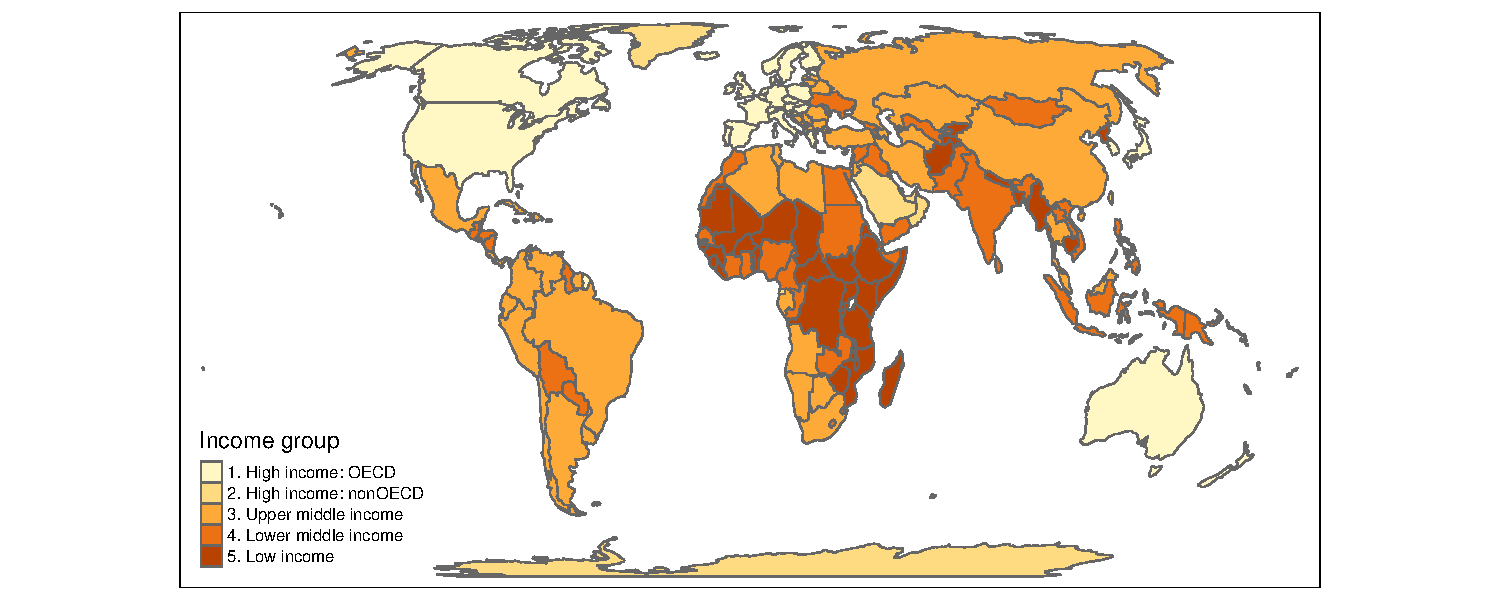
\includegraphics{tmap_files/figure-beamer/unnamed-chunk-23-1.pdf}

\end{frame}

\begin{frame}{Ein Datensatz zu den Provinzen in den Niederlanden
(R-Paket \texttt{tmap})}

\begin{longtable}[]{@{}lllrrrrrrrrrrr@{}}
\toprule
& code & name & population & pop\_men & pop\_women & pop\_0\_14 &
pop\_15\_24 & pop\_25\_44 & pop\_45\_64 & pop\_65plus & origin\_native &
origin\_west & origin\_non\_west\tabularnewline
\midrule
\endhead
0 & 20 & Groningen & 582705 & 289795 & 292875 & 15 & 15 & 25 & 27 & 18 &
87 & 7 & 6\tabularnewline
1 & 21 & Friesland & 646290 & 323215 & 323055 & 17 & 12 & 24 & 28 & 19 &
91 & 5 & 4\tabularnewline
2 & 22 & Drenthe & 488970 & 242225 & 246755 & 17 & 10 & 22 & 30 & 21 &
91 & 6 & 3\tabularnewline
3 & 23 & Overijssel & 1139680 & 570185 & 569465 & 18 & 12 & 25 & 27 & 18
& 86 & 7 & 7\tabularnewline
4 & 24 & Flevoland & 399885 & 199940 & 199940 & 20 & 13 & 27 & 28 & 12 &
71 & 9 & 20\tabularnewline
5 & 25 & Gelderland & 2019635 & 997805 & 1021790 & 17 & 12 & 24 & 29 &
18 & 85 & 8 & 7\tabularnewline
\bottomrule
\end{longtable}

\end{frame}

\begin{frame}[fragile]{Niederlande - Bevölkerung in den Provinzen}

\begin{Shaded}
\begin{Highlighting}[]
\KeywordTok{qtm}\NormalTok{(NLD_prov, }\DataTypeTok{fill=}\StringTok{"population"}\NormalTok{,}\DataTypeTok{fill.title=}\StringTok{"population"}\NormalTok{) }
\end{Highlighting}
\end{Shaded}

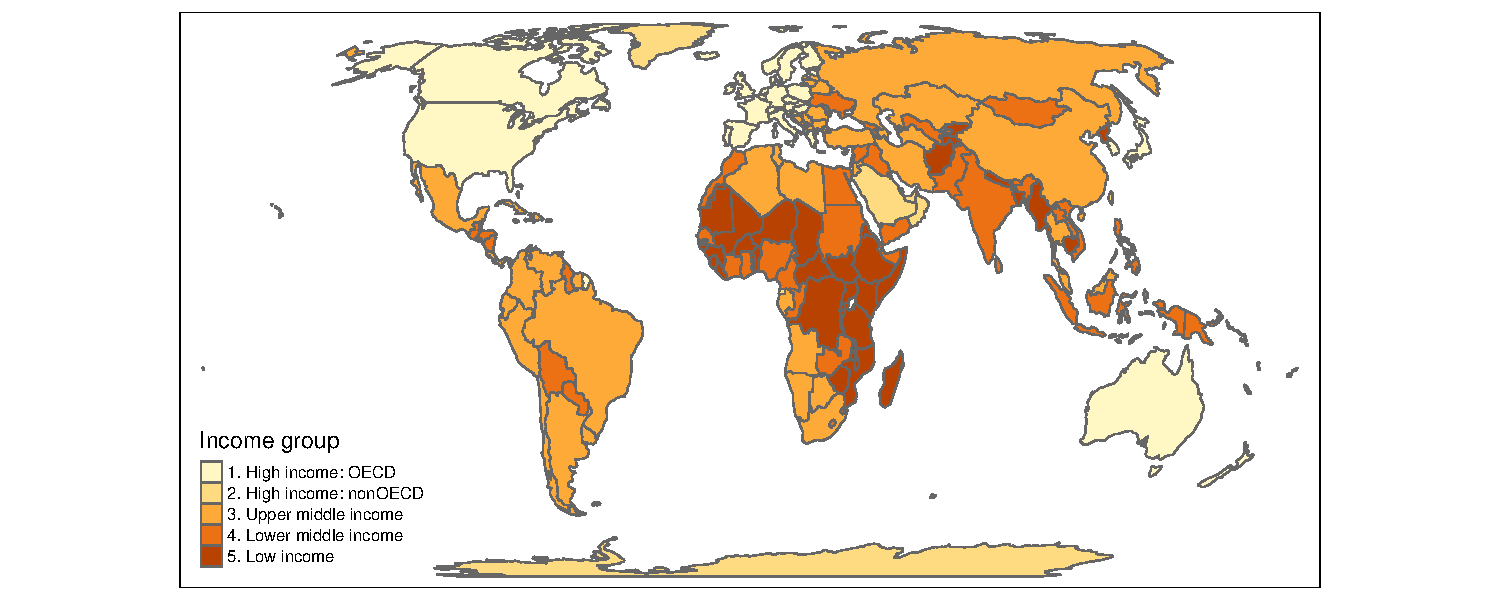
\includegraphics{tmap_files/figure-beamer/unnamed-chunk-26-1.pdf}

\end{frame}

\begin{frame}[fragile]{Anteile berechnen}

\begin{Shaded}
\begin{Highlighting}[]
\NormalTok{pop <-}\StringTok{ }\NormalTok{NLD_prov}\OperatorTok{@}\NormalTok{data}\OperatorTok{$}\NormalTok{population}
\NormalTok{pop}
\end{Highlighting}
\end{Shaded}

\begin{verbatim}
##  [1]  582705  646290  488970 1139680  399885 2019635 1253645 2741320
##  [9] 3576960  380610 2479220 1119980
\end{verbatim}

\begin{Shaded}
\begin{Highlighting}[]
\NormalTok{popmen <-}\StringTok{ }\NormalTok{NLD_prov}\OperatorTok{@}\NormalTok{data}\OperatorTok{$}\NormalTok{pop_men}
\NormalTok{popmen}
\end{Highlighting}
\end{Shaded}

\begin{verbatim}
##  [1]  289795  323215  242225  570185  199940  997805  613645 1349610
##  [9] 1764855  188655 1238600  555450
\end{verbatim}

\begin{Shaded}
\begin{Highlighting}[]
\NormalTok{prop <-}\StringTok{ }\NormalTok{popmen}\OperatorTok{/}\NormalTok{pop}
\NormalTok{prop}
\end{Highlighting}
\end{Shaded}

\begin{verbatim}
##  [1] 0.4973271 0.5001083 0.4953780 0.5003027 0.4999937 0.4940521 0.4894887
##  [8] 0.4923212 0.4933952 0.4956649 0.4995926 0.4959464
\end{verbatim}

\end{frame}

\begin{frame}[fragile]{Exkurs: Barplot vom Männeranteil}

\begin{Shaded}
\begin{Highlighting}[]
\KeywordTok{barplot}\NormalTok{(prop)}
\end{Highlighting}
\end{Shaded}

\begin{block}{Barplot mit Farbe}

\begin{Shaded}
\begin{Highlighting}[]
\KeywordTok{barplot}\NormalTok{(prop,}\DataTypeTok{col=}\StringTok{"blue"}\NormalTok{)}
\end{Highlighting}
\end{Shaded}

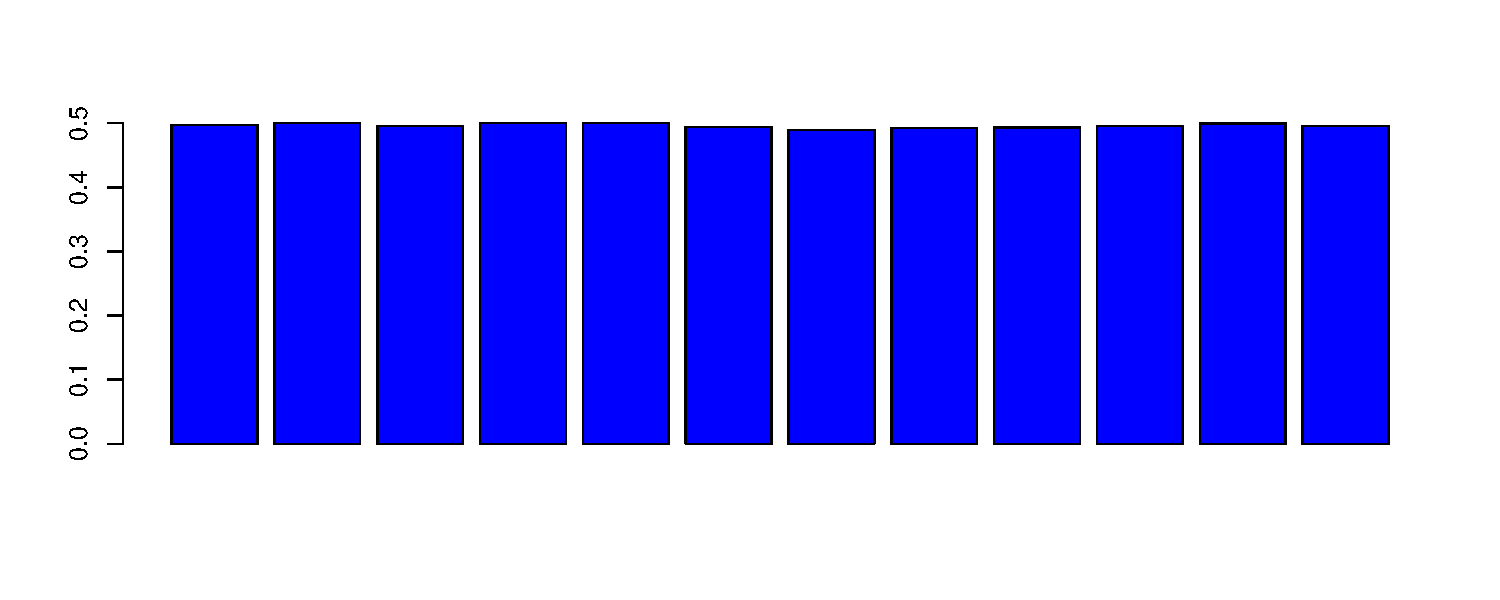
\includegraphics{tmap_files/figure-beamer/unnamed-chunk-31-1.pdf}

\end{block}

\end{frame}

\begin{frame}[fragile]{Niederlnade - Anteil Männer}

Information in Datensatz einspeisen

\begin{Shaded}
\begin{Highlighting}[]
\NormalTok{NLD_prov}\OperatorTok{@}\NormalTok{data}\OperatorTok{$}\NormalTok{proportion <-}\StringTok{ }\NormalTok{prop}
\end{Highlighting}
\end{Shaded}

\begin{Shaded}
\begin{Highlighting}[]
\KeywordTok{qtm}\NormalTok{(NLD_prov, }\DataTypeTok{fill=}\StringTok{"proportion"}\NormalTok{,}\DataTypeTok{fill.title=}\StringTok{"proportion"}\NormalTok{) }
\end{Highlighting}
\end{Shaded}

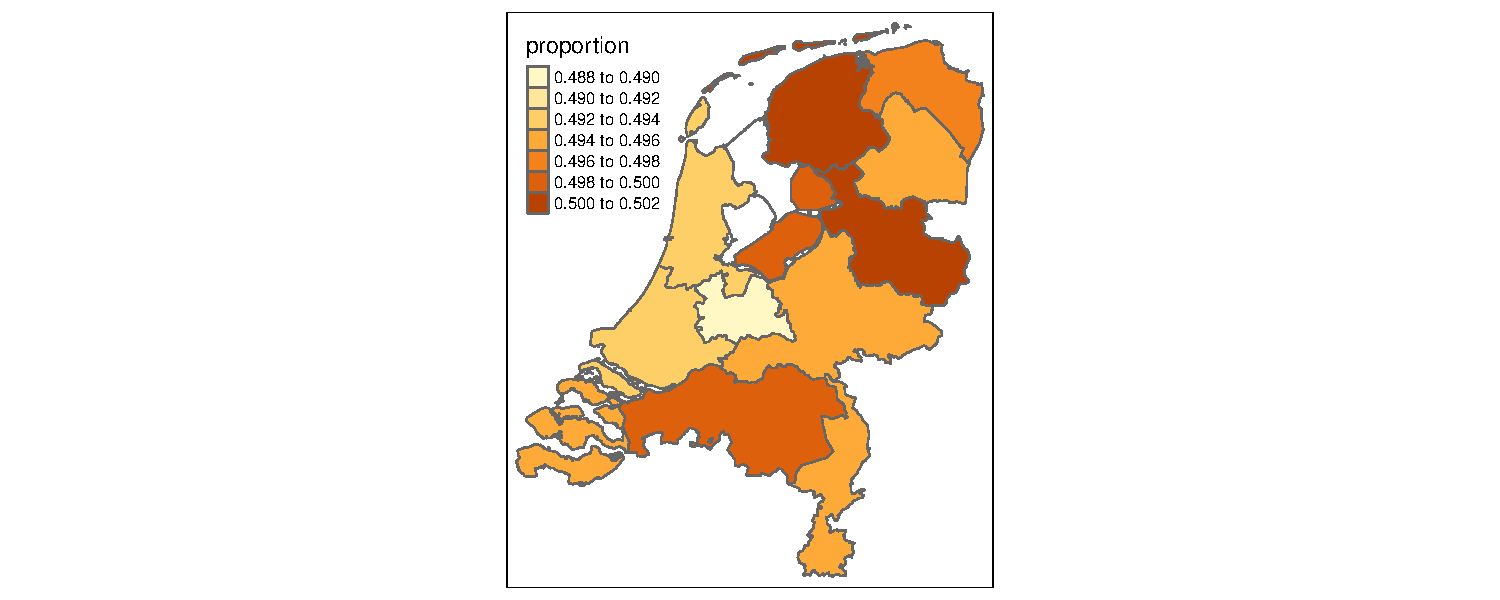
\includegraphics{tmap_files/figure-beamer/unnamed-chunk-33-1.pdf}

\end{frame}

\begin{frame}[fragile]{Ein Datensatz zu den Gemeinden in den
Niederlanden}

\begin{Shaded}
\begin{Highlighting}[]
\KeywordTok{data}\NormalTok{(NLD_muni)}
\end{Highlighting}
\end{Shaded}

\begin{longtable}[]{@{}lllr@{}}
\toprule
& name & province & population\tabularnewline
\midrule
\endhead
0 & Appingedam & Groningen & 12065\tabularnewline
1 & Bedum & Groningen & 10495\tabularnewline
2 & Bellingwedde & Groningen & 8920\tabularnewline
3 & Ten Boer & Groningen & 7480\tabularnewline
4 & Delfzijl & Groningen & 25695\tabularnewline
5 & Groningen & Groningen & 198315\tabularnewline
6 & Grootegast & Groningen & 12165\tabularnewline
7 & Haren & Groningen & 18780\tabularnewline
8 & Hoogezand-Sappemeer & Groningen & 34305\tabularnewline
9 & Leek & Groningen & 19595\tabularnewline
10 & Loppersum & Groningen & 10195\tabularnewline
11 & Marum & Groningen & 10375\tabularnewline
12 & Almere & Flevoland & 196010\tabularnewline
13 & Stadskanaal & Groningen & 32800\tabularnewline
14 & Slochteren & Groningen & 15545\tabularnewline
15 & Veendam & Groningen & 27790\tabularnewline
16 & Vlagtwedde & Groningen & 15905\tabularnewline
17 & Zeewolde & Flevoland & 21500\tabularnewline
18 & Winsum & Groningen & 13850\tabularnewline
19 & Zuidhorn & Groningen & 18775\tabularnewline
20 & Dongeradeel & Friesland & 24160\tabularnewline
21 & Achtkarspelen & Friesland & 28015\tabularnewline
22 & Ameland & Friesland & 3575\tabularnewline
23 & het Bildt & Friesland & 10625\tabularnewline
24 & Franekeradeel & Friesland & 20445\tabularnewline
25 & Harlingen & Friesland & 15820\tabularnewline
26 & Heerenveen & Friesland & 49900\tabularnewline
27 & Kollumerland en Nieuwkruisland & Friesland & 12875\tabularnewline
28 & Leeuwarden & Friesland & 107340\tabularnewline
29 & Leeuwarderadeel & Friesland & 10275\tabularnewline
30 & Ooststellingwerf & Friesland & 25670\tabularnewline
31 & Opsterland & Friesland & 29860\tabularnewline
32 & Schiermonnikoog & Friesland & 940\tabularnewline
33 & Smallingerland & Friesland & 55465\tabularnewline
34 & Terschelling & Friesland & 4780\tabularnewline
35 & Vlieland & Friesland & 1110\tabularnewline
36 & Weststellingwerf & Friesland & 25455\tabularnewline
37 & Assen & Drenthe & 67190\tabularnewline
38 & Coevorden & Drenthe & 35770\tabularnewline
39 & Emmen & Drenthe & 108050\tabularnewline
40 & Hoogeveen & Drenthe & 54665\tabularnewline
41 & Meppel & Drenthe & 32865\tabularnewline
42 & Littenseradiel & Friesland & 10925\tabularnewline
43 & Almelo & Overijssel & 72460\tabularnewline
44 & Borne & Overijssel & 21885\tabularnewline
45 & Dalfsen & Overijssel & 27675\tabularnewline
46 & Deventer & Overijssel & 98320\tabularnewline
47 & Enschede & Overijssel & 158585\tabularnewline
48 & Haaksbergen & Overijssel & 24345\tabularnewline
49 & Hardenberg & Overijssel & 59575\tabularnewline
50 & Hellendoorn & Overijssel & 35710\tabularnewline
51 & Hengelo & Overijssel & 80955\tabularnewline
52 & Kampen & Overijssel & 51090\tabularnewline
53 & Losser & Overijssel & 22610\tabularnewline
54 & Noordoostpolder & Flevoland & 46355\tabularnewline
55 & Oldenzaal & Overijssel & 32135\tabularnewline
56 & Ommen & Overijssel & 17360\tabularnewline
57 & Raalte & Overijssel & 36520\tabularnewline
58 & Staphorst & Overijssel & 16365\tabularnewline
59 & Tubbergen & Overijssel & 21205\tabularnewline
60 & Urk & Flevoland & 19470\tabularnewline
61 & Wierden & Overijssel & 23910\tabularnewline
62 & Zwolle & Overijssel & 123160\tabularnewline
63 & Rijnwaarden & Gelderland & 10915\tabularnewline
64 & Aalten & Gelderland & 27010\tabularnewline
65 & Apeldoorn & Gelderland & 157545\tabularnewline
66 & Arnhem & Gelderland & 150820\tabularnewline
67 & Barneveld & Gelderland & 54150\tabularnewline
68 & Beuningen & Gelderland & 25285\tabularnewline
69 & Brummen & Gelderland & 21175\tabularnewline
70 & Buren & Gelderland & 26020\tabularnewline
71 & Culemborg & Gelderland & 27590\tabularnewline
72 & Doesburg & Gelderland & 11435\tabularnewline
73 & Doetinchem & Gelderland & 56345\tabularnewline
74 & Druten & Gelderland & 18210\tabularnewline
75 & Duiven & Gelderland & 25610\tabularnewline
76 & Ede & Gelderland & 110655\tabularnewline
77 & Elburg & Gelderland & 22645\tabularnewline
78 & Epe & Gelderland & 32350\tabularnewline
79 & Ermelo & Gelderland & 26045\tabularnewline
80 & Geldermalsen & Gelderland & 26300\tabularnewline
81 & Groesbeek & Gelderland & 18975\tabularnewline
82 & Harderwijk & Gelderland & 45730\tabularnewline
83 & Hattem & Gelderland & 11730\tabularnewline
84 & Heerde & Gelderland & 18490\tabularnewline
85 & Heumen & Gelderland & 16335\tabularnewline
86 & Lochem & Gelderland & 33245\tabularnewline
87 & Maasdriel & Gelderland & 24155\tabularnewline
88 & Millingen aan de Rijn & Gelderland & 5875\tabularnewline
89 & Nijkerk & Gelderland & 40635\tabularnewline
90 & Nijmegen & Gelderland & 168290\tabularnewline
91 & Oldebroek & Gelderland & 22835\tabularnewline
92 & Putten & Gelderland & 23870\tabularnewline
93 & Renkum & Gelderland & 31580\tabularnewline
94 & Rheden & Gelderland & 43640\tabularnewline
95 & Rozendaal & Gelderland & 1500\tabularnewline
96 & Scherpenzeel & Gelderland & 9495\tabularnewline
97 & Tiel & Gelderland & 41775\tabularnewline
98 & Ubbergen & Gelderland & 9450\tabularnewline
99 & Voorst & Gelderland & 23765\tabularnewline
100 & Wageningen & Gelderland & 37430\tabularnewline
101 & Westervoort & Gelderland & 15135\tabularnewline
102 & Winterswijk & Gelderland & 28880\tabularnewline
103 & Wijchen & Gelderland & 41040\tabularnewline
104 & Zaltbommel & Gelderland & 27180\tabularnewline
105 & Zevenaar & Gelderland & 32280\tabularnewline
106 & Zutphen & Gelderland & 47165\tabularnewline
107 & Nunspeet & Gelderland & 26680\tabularnewline
108 & Dronten & Flevoland & 40410\tabularnewline
109 & Neerijnen & Gelderland & 12020\tabularnewline
110 & Amersfoort & Utrecht & 150895\tabularnewline
111 & Baarn & Utrecht & 24315\tabularnewline
112 & De Bilt & Utrecht & 42035\tabularnewline
113 & Bunnik & Utrecht & 14625\tabularnewline
114 & Bunschoten & Utrecht & 20490\tabularnewline
115 & Eemnes & Utrecht & 8780\tabularnewline
116 & Houten & Utrecht & 48420\tabularnewline
117 & Leusden & Utrecht & 28995\tabularnewline
118 & Lopik & Utrecht & 14000\tabularnewline
119 & Montfoort & Utrecht & 13640\tabularnewline
120 & Renswoude & Utrecht & 4925\tabularnewline
121 & Rhenen & Utrecht & 19115\tabularnewline
122 & Soest & Utrecht & 45490\tabularnewline
123 & Utrecht & Utrecht & 328165\tabularnewline
124 & Veenendaal & Utrecht & 63250\tabularnewline
125 & Woudenberg & Utrecht & 12420\tabularnewline
126 & Wijk bij Duurstede & Utrecht & 23040\tabularnewline
127 & IJsselstein & Utrecht & 34275\tabularnewline
128 & Zeist & Utrecht & 61250\tabularnewline
129 & Nieuwegein & Utrecht & 61035\tabularnewline
130 & Aalsmeer & Noord-Holland & 30760\tabularnewline
131 & Alkmaar & Noord-Holland & 94865\tabularnewline
132 & Amstelveen & Noord-Holland & 85015\tabularnewline
133 & Amsterdam & Noord-Holland & 810935\tabularnewline
134 & Graft-De Rijp & Noord-Holland & 6450\tabularnewline
135 & Beemster & Noord-Holland & 8910\tabularnewline
136 & Bergen (NH.) & Noord-Holland & 30075\tabularnewline
137 & Beverwijk & Noord-Holland & 40090\tabularnewline
138 & Blaricum & Noord-Holland & 9095\tabularnewline
139 & Bloemendaal & Noord-Holland & 22060\tabularnewline
140 & Bussum & Noord-Holland & 32630\tabularnewline
141 & Castricum & Noord-Holland & 34285\tabularnewline
142 & Diemen & Noord-Holland & 25930\tabularnewline
143 & Edam-Volendam & Noord-Holland & 28920\tabularnewline
144 & Enkhuizen & Noord-Holland & 18375\tabularnewline
145 & Haarlem & Noord-Holland & 155145\tabularnewline
146 & Haarlemmerliede en Spaarnwoude & Noord-Holland &
5535\tabularnewline
147 & Haarlemmermeer & Noord-Holland & 144060\tabularnewline
148 & Heemskerk & Noord-Holland & 39085\tabularnewline
149 & Heemstede & Noord-Holland & 26365\tabularnewline
150 & Heerhugowaard & Noord-Holland & 53305\tabularnewline
151 & Heiloo & Noord-Holland & 22635\tabularnewline
152 & Den Helder & Noord-Holland & 56595\tabularnewline
153 & Hilversum & Noord-Holland & 86425\tabularnewline
154 & Hoorn & Noord-Holland & 71700\tabularnewline
155 & Huizen & Noord-Holland & 41245\tabularnewline
156 & Landsmeer & Noord-Holland & 10445\tabularnewline
157 & Langedijk & Noord-Holland & 26935\tabularnewline
158 & Laren & Noord-Holland & 10860\tabularnewline
159 & Medemblik & Noord-Holland & 43320\tabularnewline
160 & Muiden & Noord-Holland & 6285\tabularnewline
161 & Naarden & Noord-Holland & 17205\tabularnewline
162 & Oostzaan & Noord-Holland & 9140\tabularnewline
163 & Opmeer & Noord-Holland & 11365\tabularnewline
164 & Ouder-Amstel & Noord-Holland & 13270\tabularnewline
165 & Purmerend & Noord-Holland & 79575\tabularnewline
166 & Schagen & Noord-Holland & 45975\tabularnewline
167 & Texel & Noord-Holland & 13550\tabularnewline
168 & Uitgeest & Noord-Holland & 13235\tabularnewline
169 & Uithoorn & Noord-Holland & 28415\tabularnewline
170 & Velsen & Noord-Holland & 67220\tabularnewline
171 & Weesp & Noord-Holland & 18170\tabularnewline
172 & Schermer & Noord-Holland & 5540\tabularnewline
173 & Zandvoort & Noord-Holland & 16575\tabularnewline
174 & Zeevang & Noord-Holland & 6340\tabularnewline
175 & Zaanstad & Noord-Holland & 150595\tabularnewline
176 & Alblasserdam & Zuid-Holland & 19800\tabularnewline
177 & Alphen aan den Rijn & Zuid-Holland & 106785\tabularnewline
178 & Barendrecht & Zuid-Holland & 47375\tabularnewline
179 & Bergambacht & Zuid-Holland & 9970\tabularnewline
180 & Drechterland & Noord-Holland & 19250\tabularnewline
181 & Brielle & Zuid-Holland & 16310\tabularnewline
182 & Capelle aan den IJssel & Zuid-Holland & 66175\tabularnewline
183 & Delft & Zuid-Holland & 100045\tabularnewline
184 & Dordrecht & Zuid-Holland & 118690\tabularnewline
185 & Gorinchem & Zuid-Holland & 35240\tabularnewline
186 & Gouda & Zuid-Holland & 70940\tabularnewline
187 & 's-Gravenhage & Zuid-Holland & 508940\tabularnewline
188 & Hardinxveld-Giessendam & Zuid-Holland & 17755\tabularnewline
189 & Hellevoetsluis & Zuid-Holland & 38950\tabularnewline
190 & Hendrik-Ido-Ambacht & Zuid-Holland & 28910\tabularnewline
191 & Stede Broec & Noord-Holland & 21485\tabularnewline
192 & Hillegom & Zuid-Holland & 20945\tabularnewline
193 & Katwijk & Zuid-Holland & 62780\tabularnewline
194 & Krimpen aan den IJssel & Zuid-Holland & 28825\tabularnewline
195 & Leerdam & Zuid-Holland & 20590\tabularnewline
196 & Leiden & Zuid-Holland & 121160\tabularnewline
197 & Leiderdorp & Zuid-Holland & 26810\tabularnewline
198 & Lisse & Zuid-Holland & 22335\tabularnewline
199 & Maassluis & Zuid-Holland & 32080\tabularnewline
200 & Bernisse & Zuid-Holland & 12365\tabularnewline
201 & Nieuwkoop & Zuid-Holland & 27105\tabularnewline
202 & Noordwijk & Zuid-Holland & 25690\tabularnewline
203 & Noordwijkerhout & Zuid-Holland & 15955\tabularnewline
204 & Oegstgeest & Zuid-Holland & 22910\tabularnewline
205 & Oud-Beijerland & Zuid-Holland & 23715\tabularnewline
206 & Binnenmaas & Zuid-Holland & 28710\tabularnewline
207 & Korendijk & Zuid-Holland & 10700\tabularnewline
208 & Oudewater & Utrecht & 9870\tabularnewline
209 & Papendrecht & Zuid-Holland & 32115\tabularnewline
210 & Ridderkerk & Zuid-Holland & 45250\tabularnewline
211 & Rotterdam & Zuid-Holland & 618355\tabularnewline
212 & Rijswijk & Zuid-Holland & 47635\tabularnewline
213 & Schiedam & Zuid-Holland & 76450\tabularnewline
214 & Schoonhoven & Zuid-Holland & 11900\tabularnewline
215 & Sliedrecht & Zuid-Holland & 24525\tabularnewline
216 & Cromstrijen & Zuid-Holland & 12735\tabularnewline
217 & Spijkenisse & Zuid-Holland & 72560\tabularnewline
218 & Albrandswaard & Zuid-Holland & 25070\tabularnewline
219 & Westvoorne & Zuid-Holland & 13965\tabularnewline
220 & Strijen & Zuid-Holland & 8680\tabularnewline
221 & Vianen & Utrecht & 19595\tabularnewline
222 & Vlaardingen & Zuid-Holland & 70980\tabularnewline
223 & Vlist & Zuid-Holland & 9695\tabularnewline
224 & Voorschoten & Zuid-Holland & 24950\tabularnewline
225 & Waddinxveen & Zuid-Holland & 25505\tabularnewline
226 & Wassenaar & Zuid-Holland & 25675\tabularnewline
227 & Woerden & Utrecht & 50575\tabularnewline
228 & Zoetermeer & Zuid-Holland & 123560\tabularnewline
229 & Zoeterwoude & Zuid-Holland & 8075\tabularnewline
230 & Zwijndrecht & Zuid-Holland & 44545\tabularnewline
231 & Nederlek & Zuid-Holland & 14075\tabularnewline
232 & Ouderkerk & Zuid-Holland & 8210\tabularnewline
233 & Borsele & Zeeland & 22580\tabularnewline
234 & Goes & Zeeland & 36955\tabularnewline
235 & West Maas en Waal & Gelderland & 18420\tabularnewline
236 & Hulst & Zeeland & 27385\tabularnewline
237 & Kapelle & Zeeland & 12500\tabularnewline
238 & Middelburg & Zeeland & 47640\tabularnewline
239 & Giessenlanden & Zuid-Holland & 14440\tabularnewline
240 & Reimerswaal & Zeeland & 21925\tabularnewline
241 & Zederik & Zuid-Holland & 13655\tabularnewline
242 & Terneuzen & Zeeland & 54710\tabularnewline
243 & Tholen & Zeeland & 25405\tabularnewline
244 & Veere & Zeeland & 21865\tabularnewline
245 & Vlissingen & Zeeland & 44445\tabularnewline
246 & Lingewaal & Gelderland & 11060\tabularnewline
247 & De Ronde Venen & Utrecht & 42640\tabularnewline
248 & Tytsjerksteradiel & Friesland & 31970\tabularnewline
249 & Aalburg & Noord-Brabant & 12845\tabularnewline
250 & Asten & Noord-Brabant & 16440\tabularnewline
251 & Baarle-Nassau & Noord-Brabant & 6610\tabularnewline
252 & Bergen op Zoom & Noord-Brabant & 66420\tabularnewline
253 & Best & Noord-Brabant & 28615\tabularnewline
254 & Boekel & Noord-Brabant & 10090\tabularnewline
255 & Boxmeer & Noord-Brabant & 28145\tabularnewline
256 & Boxtel & Noord-Brabant & 30320\tabularnewline
257 & Breda & Noord-Brabant & 179620\tabularnewline
258 & Deurne & Noord-Brabant & 31660\tabularnewline
259 & Pekela & Groningen & 12705\tabularnewline
260 & Dongen & Noord-Brabant & 25355\tabularnewline
261 & Eersel & Noord-Brabant & 18180\tabularnewline
262 & Eindhoven & Noord-Brabant & 220920\tabularnewline
263 & Etten-Leur & Noord-Brabant & 42355\tabularnewline
264 & Geertruidenberg & Noord-Brabant & 21570\tabularnewline
265 & Gilze en Rijen & Noord-Brabant & 26070\tabularnewline
266 & Goirle & Noord-Brabant & 23095\tabularnewline
267 & Grave & Noord-Brabant & 12695\tabularnewline
268 & Haaren & Noord-Brabant & 13585\tabularnewline
269 & Helmond & Noord-Brabant & 89255\tabularnewline
270 & 's-Hertogenbosch & Noord-Brabant & 143730\tabularnewline
271 & Heusden & Noord-Brabant & 43165\tabularnewline
272 & Hilvarenbeek & Noord-Brabant & 15090\tabularnewline
273 & Loon op Zand & Noord-Brabant & 23080\tabularnewline
274 & Mill en Sint Hubert & Noord-Brabant & 10850\tabularnewline
275 & Nuenen. Gerwen en Nederwetten & Noord-Brabant &
22620\tabularnewline
276 & Oirschot & Noord-Brabant & 17980\tabularnewline
277 & Oisterwijk & Noord-Brabant & 25800\tabularnewline
278 & Oosterhout & Noord-Brabant & 53715\tabularnewline
279 & Oss & Noord-Brabant & 84955\tabularnewline
280 & Rucphen & Noord-Brabant & 22180\tabularnewline
281 & Schijndel & Noord-Brabant & 23360\tabularnewline
282 & Sint-Michielsgestel & Noord-Brabant & 28120\tabularnewline
283 & Sint-Oedenrode & Noord-Brabant & 17935\tabularnewline
284 & Someren & Noord-Brabant & 18690\tabularnewline
285 & Son en Breugel & Noord-Brabant & 16235\tabularnewline
286 & Steenbergen & Noord-Brabant & 23375\tabularnewline
287 & Waterland & Noord-Holland & 17135\tabularnewline
288 & Tilburg & Noord-Brabant & 210270\tabularnewline
289 & Uden & Noord-Brabant & 40910\tabularnewline
290 & Valkenswaard & Noord-Brabant & 30335\tabularnewline
291 & Veghel & Noord-Brabant & 37465\tabularnewline
292 & Veldhoven & Noord-Brabant & 44155\tabularnewline
293 & Vught & Noord-Brabant & 25635\tabularnewline
294 & Waalre & Noord-Brabant & 16765\tabularnewline
295 & Waalwijk & Noord-Brabant & 46495\tabularnewline
296 & Werkendam & Noord-Brabant & 26385\tabularnewline
297 & Woensdrecht & Noord-Brabant & 21620\tabularnewline
298 & Woudrichem & Noord-Brabant & 14425\tabularnewline
299 & Zundert & Noord-Brabant & 21400\tabularnewline
300 & Wormerland & Noord-Holland & 15775\tabularnewline
301 & Onderbanken & Limburg & 7880\tabularnewline
302 & Landgraaf & Limburg & 37570\tabularnewline
303 & Beek & Limburg & 16270\tabularnewline
304 & Beesel & Limburg & 13615\tabularnewline
305 & Bergen (L.) & Limburg & 13235\tabularnewline
306 & Brunssum & Limburg & 28955\tabularnewline
307 & Gennep & Limburg & 17285\tabularnewline
308 & Heerlen & Limburg & 88260\tabularnewline
309 & Kerkrade & Limburg & 46785\tabularnewline
310 & Maastricht & Limburg & 122485\tabularnewline
311 & Meerssen & Limburg & 19255\tabularnewline
312 & Mook en Middelaar & Limburg & 7795\tabularnewline
313 & Nederweert & Limburg & 16750\tabularnewline
314 & Nuth & Limburg & 15580\tabularnewline
315 & Roermond & Limburg & 56930\tabularnewline
316 & Schinnen & Limburg & 12900\tabularnewline
317 & Simpelveld & Limburg & 10845\tabularnewline
318 & Stein & Limburg & 25390\tabularnewline
319 & Vaals & Limburg & 9685\tabularnewline
320 & Venlo & Limburg & 100425\tabularnewline
321 & Venray & Limburg & 43110\tabularnewline
322 & Voerendaal & Limburg & 12455\tabularnewline
323 & Weert & Limburg & 48720\tabularnewline
324 & Valkenburg aan de Geul & Limburg & 16675\tabularnewline
325 & Lelystad & Flevoland & 76140\tabularnewline
326 & Horst aan de Maas & Limburg & 41725\tabularnewline
327 & Oude IJsselstreek & Gelderland & 39595\tabularnewline
328 & Teylingen & Zuid-Holland & 35735\tabularnewline
329 & Utrechtse Heuvelrug & Utrecht & 47950\tabularnewline
330 & Oost Gelre & Gelderland & 29700\tabularnewline
331 & Koggenland & Noord-Holland & 22485\tabularnewline
332 & Lansingerland & Zuid-Holland & 57120\tabularnewline
333 & Leudal & Limburg & 36220\tabularnewline
334 & Maasgouw & Limburg & 23905\tabularnewline
335 & Eemsmond & Groningen & 15925\tabularnewline
336 & Gemert-Bakel & Noord-Brabant & 29315\tabularnewline
337 & Halderberge & Noord-Brabant & 29340\tabularnewline
338 & Heeze-Leende & Noord-Brabant & 15350\tabularnewline
339 & Laarbeek & Noord-Brabant & 21800\tabularnewline
340 & De Marne & Groningen & 10210\tabularnewline
341 & Reusel-De Mierden & Noord-Brabant & 12710\tabularnewline
342 & Roerdalen & Limburg & 20830\tabularnewline
343 & Maasdonk & Noord-Brabant & 11240\tabularnewline
344 & Roosendaal & Noord-Brabant & 77025\tabularnewline
345 & Schouwen-Duiveland & Zeeland & 33850\tabularnewline
346 & Aa en Hunze & Drenthe & 25355\tabularnewline
347 & Borger-Odoorn & Drenthe & 25625\tabularnewline
348 & Cuijk & Noord-Brabant & 24780\tabularnewline
349 & Landerd & Noord-Brabant & 15265\tabularnewline
350 & De Wolden & Drenthe & 23580\tabularnewline
351 & Noord-Beveland & Zeeland & 7530\tabularnewline
352 & Wijdemeren & Noord-Holland & 23185\tabularnewline
353 & Noordenveld & Drenthe & 31085\tabularnewline
354 & Twenterand & Overijssel & 33930\tabularnewline
355 & Westerveld & Drenthe & 18930\tabularnewline
356 & Sint Anthonis & Noord-Brabant & 11690\tabularnewline
357 & Lingewaard & Gelderland & 45775\tabularnewline
358 & Cranendonck & Noord-Brabant & 20345\tabularnewline
359 & Steenwijkerland & Overijssel & 43350\tabularnewline
360 & Moerdijk & Noord-Brabant & 36730\tabularnewline
361 & Echt-Susteren & Limburg & 31975\tabularnewline
362 & Sluis & Zeeland & 23820\tabularnewline
363 & Drimmelen & Noord-Brabant & 26695\tabularnewline
364 & Bernheze & Noord-Brabant & 29690\tabularnewline
365 & Ferwerderadiel & Friesland & 8790\tabularnewline
366 & Alphen-Chaam & Noord-Brabant & 9715\tabularnewline
367 & Bergeijk & Noord-Brabant & 18255\tabularnewline
368 & Bladel & Noord-Brabant & 19835\tabularnewline
369 & Gulpen-Wittem & Limburg & 14485\tabularnewline
370 & Tynaarlo & Drenthe & 32490\tabularnewline
371 & Midden-Drenthe & Drenthe & 33365\tabularnewline
372 & Overbetuwe & Gelderland & 46665\tabularnewline
373 & Hof van Twente & Overijssel & 34995\tabularnewline
374 & Neder-Betuwe & Gelderland & 22555\tabularnewline
375 & Rijssen-Holten & Overijssel & 37660\tabularnewline
376 & Geldrop-Mierlo & Noord-Brabant & 38855\tabularnewline
377 & Olst-Wijhe & Overijssel & 17770\tabularnewline
378 & Dinkelland & Overijssel & 25945\tabularnewline
379 & Westland & Zuid-Holland & 103240\tabularnewline
380 & Midden-Delfland & Zuid-Holland & 18455\tabularnewline
381 & Berkelland & Gelderland & 44665\tabularnewline
382 & Bronckhorst & Gelderland & 36930\tabularnewline
383 & Sittard-Geleen & Limburg & 93690\tabularnewline
384 & Kaag en Braassem & Zuid-Holland & 25745\tabularnewline
385 & Dantumadiel & Friesland & 19030\tabularnewline
386 & Zuidplas & Zuid-Holland & 40890\tabularnewline
387 & Peel en Maas & Limburg & 43315\tabularnewline
388 & Oldambt & Groningen & 38560\tabularnewline
389 & Zwartewaterland & Overijssel & 22165\tabularnewline
390 & Sudwest-Fryslan & Friesland & 84180\tabularnewline
391 & Bodegraven-Reeuwijk & Zuid-Holland & 32910\tabularnewline
392 & Eijsden-Margraten & Limburg & 24980\tabularnewline
393 & Stichtse Vecht & Utrecht & 63855\tabularnewline
394 & Menameradiel & Friesland & 13670\tabularnewline
395 & Hollands Kroon & Noord-Holland & 47500\tabularnewline
396 & Leidschendam-Voorburg & Zuid-Holland & 73355\tabularnewline
397 & De Friese Meren & Friesland & 51415\tabularnewline
398 & Goeree-Overflakkee & Zuid-Holland & 48245\tabularnewline
399 & Pijnacker-Nootdorp & Zuid-Holland & 51070\tabularnewline
400 & Molenwaard & Zuid-Holland & 29030\tabularnewline
401 & Montferland & Gelderland & 34985\tabularnewline
402 & Menterwolde & Groningen & 12255\tabularnewline
\bottomrule
\end{longtable}

\end{frame}

\begin{frame}[fragile]{Bevölkerung der Gemeinden in den Niederlanden}

\begin{Shaded}
\begin{Highlighting}[]
\KeywordTok{qtm}\NormalTok{(NLD_muni, }\DataTypeTok{fill=}\StringTok{"population"}\NormalTok{) }
\end{Highlighting}
\end{Shaded}

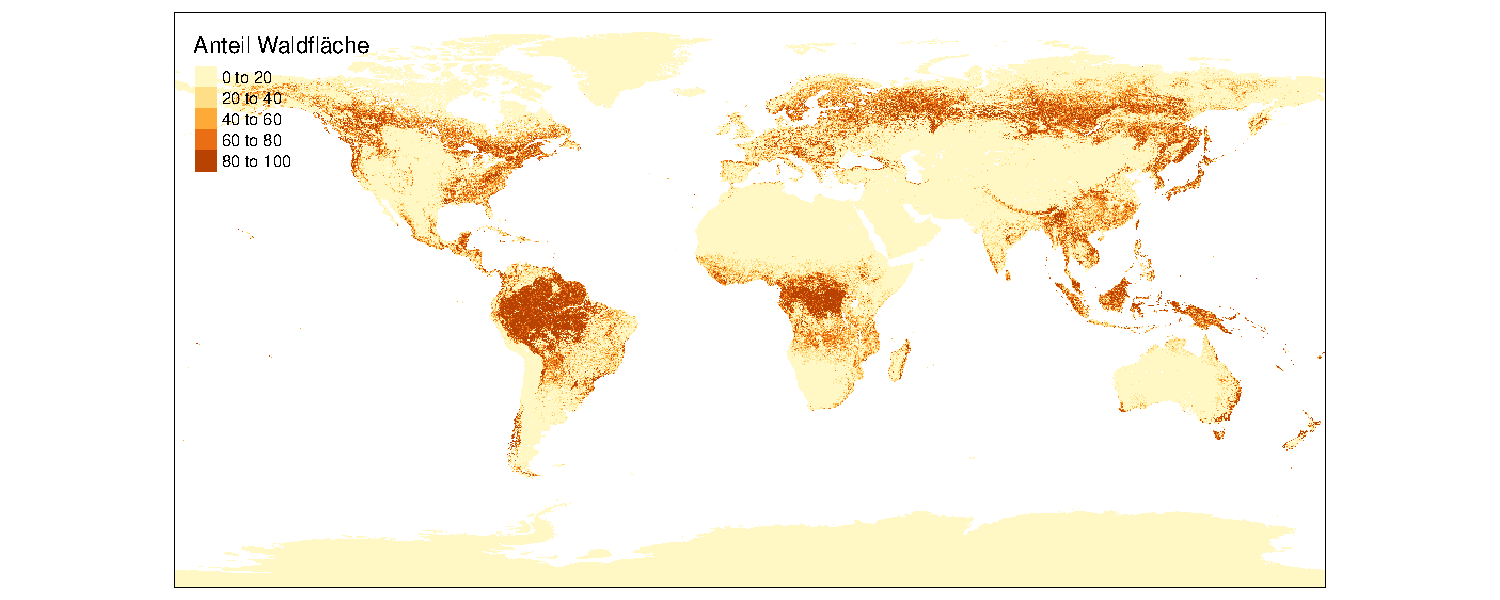
\includegraphics{tmap_files/figure-beamer/unnamed-chunk-39-1.pdf}

\end{frame}

\begin{frame}[fragile]{Zwei Karten}

\begin{Shaded}
\begin{Highlighting}[]
\KeywordTok{tm_shape}\NormalTok{(Europe) }\OperatorTok{+}
\StringTok{    }\KeywordTok{tm_fill}\NormalTok{(}\KeywordTok{c}\NormalTok{(}\StringTok{"pop_est"}\NormalTok{, }\StringTok{"economy"}\NormalTok{), }
        \DataTypeTok{title=}\KeywordTok{c}\NormalTok{(}\StringTok{"Population"}\NormalTok{, }\StringTok{"Economy"}\NormalTok{))}
\end{Highlighting}
\end{Shaded}

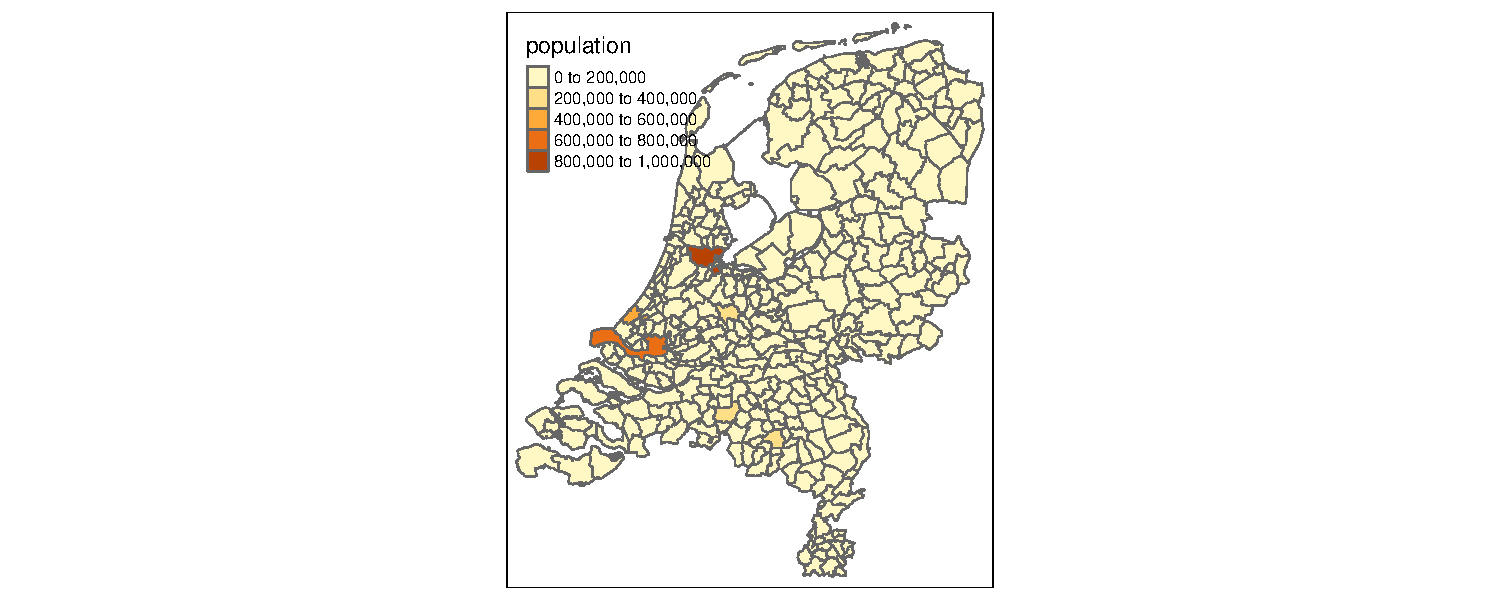
\includegraphics{tmap_files/figure-beamer/unnamed-chunk-40-1.pdf}

\end{frame}

\begin{frame}[fragile]{Räumliche Daten zur Flächennutzung}

\begin{Shaded}
\begin{Highlighting}[]
\KeywordTok{data}\NormalTok{(land)}
\KeywordTok{data}\NormalTok{(World)}
\end{Highlighting}
\end{Shaded}

\begin{longtable}[]{@{}llr@{}}
\toprule
& cover\_cls & trees\tabularnewline
\midrule
\endhead
215556 & Bare area/Sparse vegetation & 0\tabularnewline
137686 & Water & NA\tabularnewline
44785 & Water & NA\tabularnewline
88234 & Other natural vegetation & 1\tabularnewline
286270 & Water & NA\tabularnewline
146833 & Water & NA\tabularnewline
307784 & Water & NA\tabularnewline
458432 & Water & NA\tabularnewline
211482 & Forest & 96\tabularnewline
493482 & Water & NA\tabularnewline
\bottomrule
\end{longtable}

\end{frame}

\begin{frame}[fragile]{Weltweite Flächennutzung}

\begin{Shaded}
\begin{Highlighting}[]
\KeywordTok{tm_shape}\NormalTok{(land,  }\DataTypeTok{relative=}\OtherTok{FALSE}\NormalTok{) }\OperatorTok{+}
\StringTok{    }\KeywordTok{tm_raster}\NormalTok{(}\StringTok{"trees"}\NormalTok{, }\DataTypeTok{title=}\StringTok{"Anteil Waldfläche"}\NormalTok{)}
\end{Highlighting}
\end{Shaded}

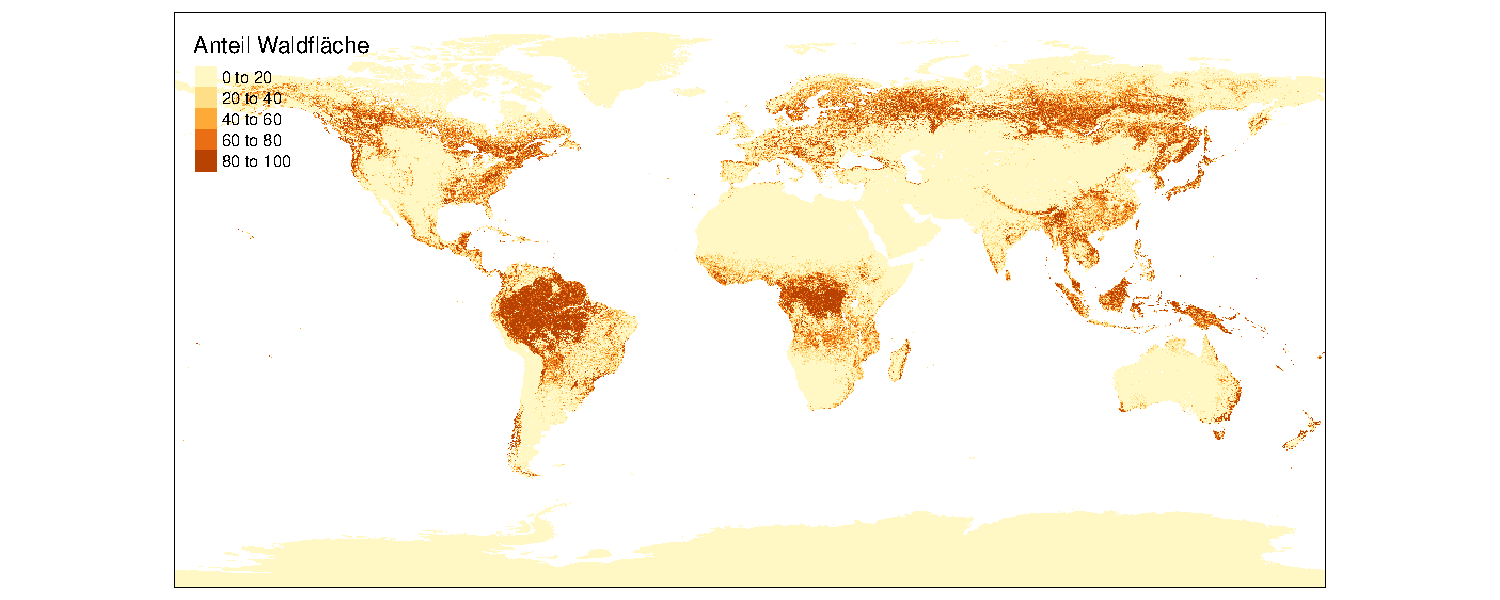
\includegraphics{tmap_files/figure-beamer/unnamed-chunk-44-1.pdf}

\end{frame}

\begin{frame}[fragile]{Räumliche Daten zu Metropolregionen}

\begin{Shaded}
\begin{Highlighting}[]
\KeywordTok{data}\NormalTok{(metro)}
\end{Highlighting}
\end{Shaded}

\begin{longtable}[]{@{}llllrrrrrrrrr@{}}
\toprule
& name & name\_long & iso\_a3 & pop1950 & pop1960 & pop1970 & pop1980 &
pop1990 & pop2000 & pop2010 & pop2020 & pop2030\tabularnewline
\midrule
\endhead
2 & Kabul & Kabul & AFG & 170784 & 285352 & 471891 & 977824 & 1549320 &
2401109 & 3722320 & 5721697 & 8279607\tabularnewline
8 & Algiers & El Djazair (Algiers) & DZA & 516450 & 871636 & 1281127 &
1621442 & 1797068 & 2140577 & 2432023 & 2835218 & 3404575\tabularnewline
13 & Luanda & Luanda & AGO & 138413 & 219427 & 459225 & 771349 & 1390240
& 2591388 & 4508434 & 6836849 & 10428756\tabularnewline
16 & Buenos Aires & Buenos Aires & ARG & 5097612 & 6597634 & 8104621 &
9422362 & 10513284 & 12406780 & 14245871 & 15894307 &
16956491\tabularnewline
17 & Cordoba & Cordoba & ARG & 429249 & 605309 & 809794 & 1009521 &
1200168 & 1347561 & 1459268 & 1562509 & 1718192\tabularnewline
25 & Rosario & Rosario & ARG & 554483 & 671349 & 816230 & 953491 &
1083819 & 1152387 & 1298073 & 1453814 & 1606993\tabularnewline
32 & Yerevan & Yerevan & ARM & 341432 & 537759 & 778158 & 1041587 &
1174524 & 1111301 & 1065597 & 1023703 & 1057459\tabularnewline
33 & Adelaide & Adelaide & AUS & 429277 & 571822 & 850168 & 971856 &
1081618 & 1141623 & 1217990 & 1320783 & 1505422\tabularnewline
34 & Brisbane & Brisbane & AUS & 441718 & 602999 & 904777 & 1134833 &
1381306 & 1666203 & 2033617 & 2388517 & 2721325\tabularnewline
37 & Melbourne & Melbourne & AUS & 1331966 & 1851220 & 2499109 & 2839019
& 3154314 & 3460541 & 3951216 & 4500501 & 5070873\tabularnewline
\bottomrule
\end{longtable}

\end{frame}

\begin{frame}[fragile]{Nur ein Land visualisieren}

\begin{Shaded}
\begin{Highlighting}[]
\KeywordTok{tm_shape}\NormalTok{(Europe[Europe}\OperatorTok{$}\NormalTok{name}\OperatorTok{==}\StringTok{"Austria"}\NormalTok{, ]) }\OperatorTok{+}
\StringTok{    }\KeywordTok{tm_polygons}\NormalTok{()}
\end{Highlighting}
\end{Shaded}

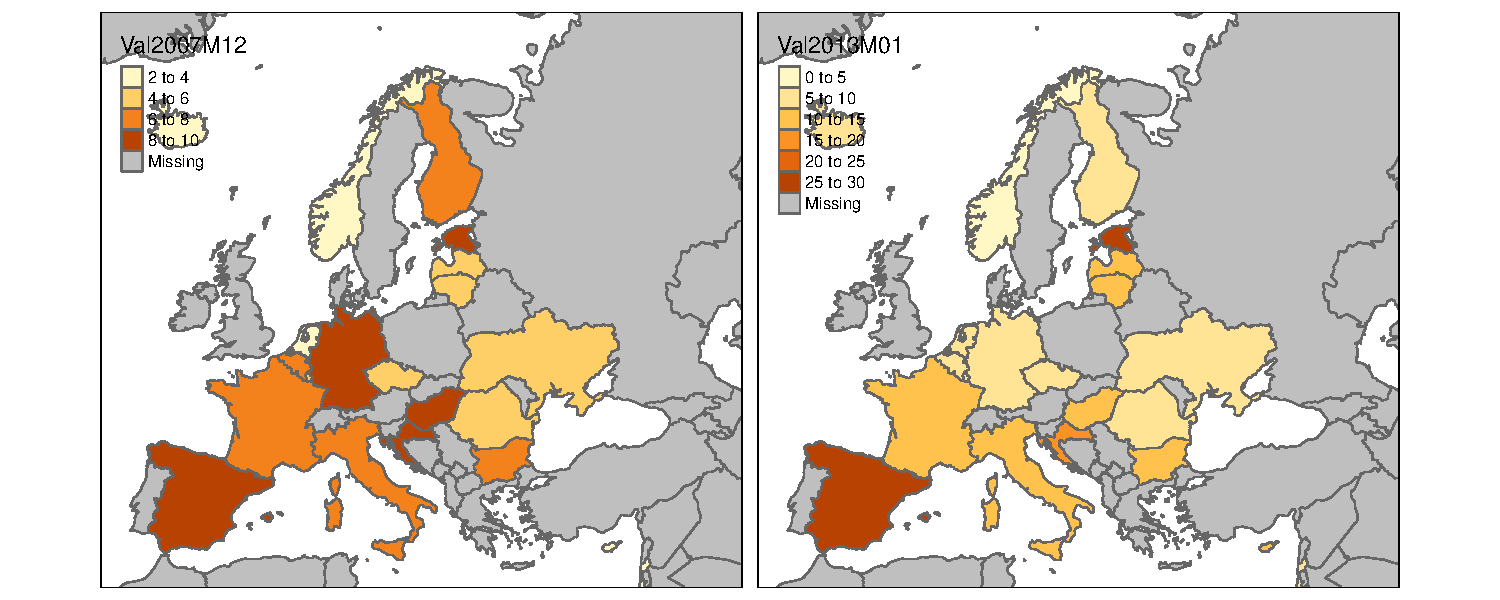
\includegraphics{tmap_files/figure-beamer/unnamed-chunk-48-1.pdf}

\end{frame}

\begin{frame}[fragile]{Beispieldaten laden}

\begin{block}{Datenquelle Eurostat}

\begin{itemize}
\tightlist
\item
  Daten zur Arbeitslosigkeit in Europa
\end{itemize}

\begin{Shaded}
\begin{Highlighting}[]
\NormalTok{url <-}\StringTok{ "https://raw.githubusercontent.com/Japhilko/}
\StringTok{GeoData/master/2015/data/Unemployment07a13.csv"}

\NormalTok{Unemp <-}\StringTok{ }\KeywordTok{read.csv}\NormalTok{(url) }
\end{Highlighting}
\end{Shaded}

\end{block}

\end{frame}

\begin{frame}{Überblick über die Daten}

\begin{longtable}[]{@{}rlrr@{}}
\toprule
X & GEO & Val2007M12 & Val2013M01\tabularnewline
\midrule
\endhead
9316 & EU28 & 6.9 & 10.9\tabularnewline
9325 & EU27 & 6.9 & 10.9\tabularnewline
9334 & EU25 & 6.9 & 11.0\tabularnewline
9343 & EU15 & 6.9 & 11.1\tabularnewline
9352 & EA & 7.3 & 12.0\tabularnewline
9361 & EA19 & 7.3 & 12.0\tabularnewline
9370 & EA18 & 7.4 & 12.0\tabularnewline
9379 & EA17 & 7.4 & 12.0\tabularnewline
9388 & EA16 & 7.4 & 12.0\tabularnewline
9397 & EA15 & 7.3 & 12.0\tabularnewline
\bottomrule
\end{longtable}

\end{frame}

\begin{frame}[fragile]{Nutzung des Paketes \texttt{tmap} mit eigenen
Daten}

\begin{Shaded}
\begin{Highlighting}[]
\KeywordTok{library}\NormalTok{(}\StringTok{"tmap"}\NormalTok{)}
\KeywordTok{data}\NormalTok{(Europe)}
\end{Highlighting}
\end{Shaded}

\begin{block}{Die Daten matchen}

\begin{Shaded}
\begin{Highlighting}[]
\NormalTok{iso_a2<-}\StringTok{ }\KeywordTok{substr}\NormalTok{(Europe}\OperatorTok{@}\NormalTok{data}\OperatorTok{$}\NormalTok{iso_a3,}\DecValTok{1}\NormalTok{,}\DecValTok{2}\NormalTok{)}
\NormalTok{ind <-}\StringTok{ }\KeywordTok{match}\NormalTok{(iso_a2,Unemp}\OperatorTok{$}\NormalTok{GEO)}
\NormalTok{Europe}\OperatorTok{@}\NormalTok{data}\OperatorTok{$}\NormalTok{Val2007M12 <-}\StringTok{ }\NormalTok{Unemp}\OperatorTok{$}\NormalTok{Val2007M12[ind]}
\NormalTok{Europe}\OperatorTok{@}\NormalTok{data}\OperatorTok{$}\NormalTok{Val2013M01 <-}\StringTok{ }\NormalTok{Unemp}\OperatorTok{$}\NormalTok{Val2013M01[ind]}
\end{Highlighting}
\end{Shaded}

\end{block}

\end{frame}

\begin{frame}[fragile]{Eine Karte erzeugen}

\begin{Shaded}
\begin{Highlighting}[]
\KeywordTok{qtm}\NormalTok{(Europe,}\KeywordTok{c}\NormalTok{(}\StringTok{"Val2007M12"}\NormalTok{,}\StringTok{"Val2013M01"}\NormalTok{))}
\end{Highlighting}
\end{Shaded}

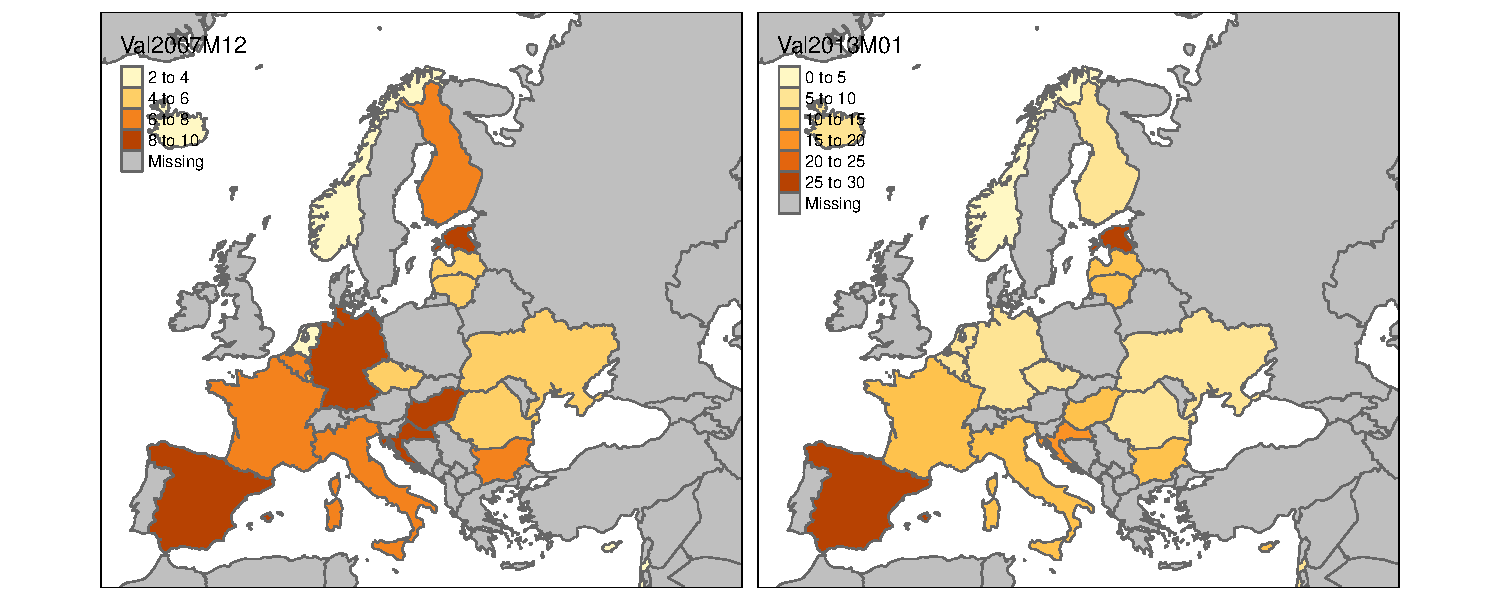
\includegraphics{tmap_files/figure-beamer/unnamed-chunk-53-1.pdf}

\end{frame}

\begin{frame}[fragile]{Kleine und viele Karten}

\begin{Shaded}
\begin{Highlighting}[]
\KeywordTok{tm_shape}\NormalTok{(Europe[Europe}\OperatorTok{$}\NormalTok{continent}\OperatorTok{==}\StringTok{"Europe"}\NormalTok{,]) }\OperatorTok{+}
\StringTok{    }\KeywordTok{tm_fill}\NormalTok{(}\StringTok{"part"}\NormalTok{, }\DataTypeTok{thres.poly =} \DecValTok{0}\NormalTok{) }\OperatorTok{+}
\StringTok{    }\KeywordTok{tm_facets}\NormalTok{(}\StringTok{"name"}\NormalTok{, }\DataTypeTok{free.coords=}\OtherTok{TRUE}\NormalTok{)}
\end{Highlighting}
\end{Shaded}

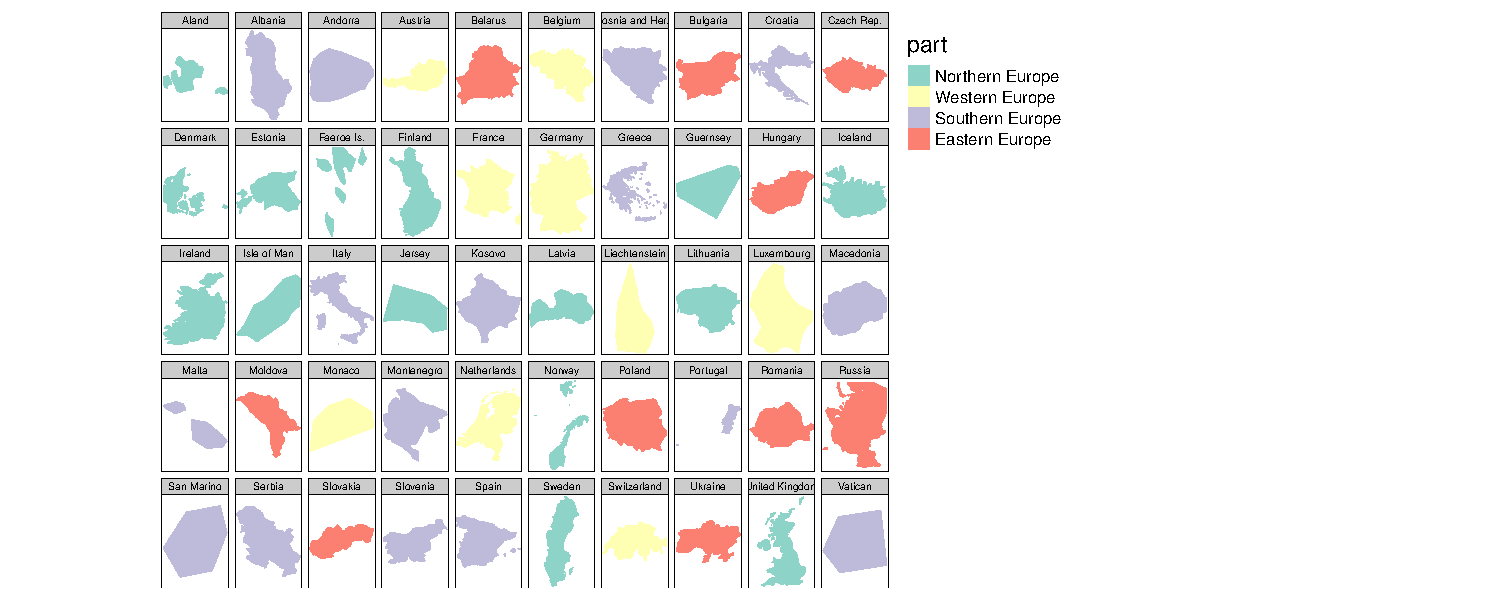
\includegraphics{tmap_files/figure-beamer/unnamed-chunk-55-1.pdf}

\end{frame}

\begin{frame}[fragile]{tmap zitieren}

\begin{Shaded}
\begin{Highlighting}[]
\KeywordTok{citation}\NormalTok{(}\StringTok{"tmap"}\NormalTok{)}
\end{Highlighting}
\end{Shaded}

\begin{verbatim}
## 
## To cite tmap/tmaptools in publications use:
## 
## Tennekes M (2018). "tmap: Thematic Maps in R." _Journal of
## Statistical Software_, *84*(6), 1-39. doi: 10.18637/jss.v084.i06
## (URL: http://doi.org/10.18637/jss.v084.i06).
## 
## A BibTeX entry for LaTeX users is
## 
##   @Article{,
##     title = {{tmap}: Thematic Maps in {R}},
##     author = {Martijn Tennekes},
##     journal = {Journal of Statistical Software},
##     year = {2018},
##     volume = {84},
##     number = {6},
##     pages = {1--39},
##     doi = {10.18637/jss.v084.i06},
##   }
\end{verbatim}

\end{frame}

\end{document}
